\documentclass{article}
\usepackage{fullpage,subfigure,fancyhdr}
\usepackage[pdftex]{color}
\usepackage{wrapfig}
\usepackage{textcomp}
\usepackage{verbatim}
\usepackage{times}
\usepackage{amsfonts,amsmath,amssymb,amsthm}
\usepackage{textcomp}
\usepackage{url}
\usepackage{mdwlist}
\usepackage{subfigure}
\usepackage{sidecap}
\usepackage{wrapfig}
\usepackage{xspace}
\usepackage{algorithm,algorithmic}
\usepackage[pdftex]{graphicx}
\usepackage[colorlinks=true,pagebackref,linkcolor=magenta]{hyperref}
\usepackage[sort&compress,comma,round,numbers]{natbib}
\usepackage{pict2e}
\usepackage[nottoc,numbib]{tocbibind}
\usepackage{paralist}
\usepackage{multicol}
\usepackage{lettrine}
\usepackage{lineno}
% \usepackage{trackchanges}
% \usepackage{mcode}

\usepackage{helvet}
\renewcommand{\familydefault}{\sfdefault}
\definecolor{MyGray}{rgb}{0.7,0.7,0.7}

% \numberwithin{figure}{section}
% \numberwithin{table}{section}
% \numberwithin{algorithm}{section}


%%%%% COLOR STUFF %%%%%%%%%%
\newcommand{\db}[1]{{\color{dark_blue}{#1}}}
\newcommand{\bb}[1]{{\textbf{\db{#1}}}}

\definecolor{MyPlum}{rgb}{0.3,0,0.3}
\definecolor{MyOrange}{rgb}{1,0.5,0}
\definecolor{deep_blue}{rgb}{0,.2,.5}
\definecolor{dark_blue}{rgb}{0,.15,.5}

\newcommand{\marta}[1]{{\color{red}{\it marta: #1}}}
\newcommand{\youngser}[1]{{\color{green}{\it youngser: #1}}}
\newcommand{\brett}[1]{{\color{blue}{\it brett says: #1}}}
\newcommand{\jovo}[1]{{\color{magenta}{\it JoVo: #1}}}
\newcommand{\rb}[1]{{\color{red}{\it rb: #1}}}
\newcommand{\bro}[1]{{\color{blue}{\it youngser: #1}}}
\newcommand{\agastya}[1]{{\color{red}{\it agastya: #1}}}
\providecommand{\tg}[1]{\textcolor{green}{#1}}
\providecommand{\tb}[1]{\textcolor{blue}{#1}}
\providecommand{\tr}[1]{\textcolor{red}{#1}}
\providecommand{\tk}[1]{\textcolor{black}{#1}}
\providecommand{\twhite}[1]{\textcolor{white}{#1}}


%%%%%%%%% MATH OPERATORS %%%%%%%%%%%%
\providecommand{\ve}[1]{\boldsymbol{#1}}
\providecommand{\ma}[1]{\boldsymbol{#1}}
\providecommand{\norm}[1]{\left \lVert#1 \right  \rVert}
\providecommand{\deter}[1]{\lvert #1 \rvert}
\providecommand{\abs}[1]{\left \lvert #1 \right \rvert}
\providecommand{\mat}[1]{\left[ #1 \right]}
\newcommand{\trans}[1]{{#1}^{\ensuremath{\mathsf{T}}}}           % transpose
\newcommand{\transpose}[1]{{#1}^{\ensuremath{\mathsf{T}}}}           % transpose
\newcommand{\argmax}{\operatornamewithlimits{argmax}}
\newcommand{\argmin}{\operatornamewithlimits{argmin}}
\newcommand{\T}{^{\ensuremath{\mathsf{T}}}}           % transpose
\newcommand{\from}{{\ensuremath{\colon}}}           % :
\newcommand{\trace}[1]{{\ensuremath{\operatorname{tr}\!\left(#1\right)}}}           % :

\providecommand{\ms}[1]{\mathsf{#1}}
\providecommand{\mc}[1]{\mathcal{#1}}
\providecommand{\mb}[1]{\boldsymbol{#1}}
\providecommand{\mbb}[1]{\mathbb{#1}}
\providecommand{\mv}[1]{\vec{#1}}
\providecommand{\mh}[1]{\hat{#1}}
\providecommand{\wh}[1]{\widehat{#1}}
\providecommand{\mhv}[1]{\mh{\mv{#1}}}
\providecommand{\mvh}[1]{\mv{\mh{#1}}}
\providecommand{\mt}[1]{\widetilde{#1}}
\providecommand{\mhc}[1]{\hat{\mathcal{#1}}}
\providecommand{\mbc}[1]{\mb{\mathcal{#1}}}
\providecommand{\mvc}[1]{\mv{\mathcal{#1}}}
\providecommand{\mtc}[1]{\widetilde{\mathcal{#1}}}
\providecommand{\mth}[1]{\mt{\mh{#1}}}
\providecommand{\mht}[1]{\mh{\mt{#1}}}
\providecommand{\mhb}[1]{\hat{\boldsymbol{#1}}}
\providecommand{\whb}[1]{\widehat{\boldsymbol{#1}}}
\providecommand{\mvb}[1]{\vec{\boldsymbol{#1}}}
\providecommand{\mtb}[1]{\widetilde{\boldsymbol{#1}}}
\providecommand{\mbt}[1]{\widetilde{\boldsymbol{#1}}}
\providecommand{\mvc}[1]{\vec{\mathcal{#1}}}
% \newcommand{\D}[2]{\frac{\partial #1}{\partial #2}}
\newcommand{\dd}[2]{\frac{\partial ^2 #1}{\partial #2 ^2}}
\newcommand{\DDD}[3]{\frac{\partial ^2 #1}{\partial #2 \partial #3}}
\newcommand{\Di}[2]{\frac{\partial ^i #1}{\partial #2 ^i}}



%%%%%%%%%% SECTIONS & STUFF %%%%%%%%%%%%%

\newtheorem{Rem}{Remark}%[section]
\newtheorem{Alg}{Algorithm}%[section]
\newtheorem{thm}{Theorem}
\newtheorem{lem}{Lemma}
\newtheorem{Thm}{Theorem}[section]
\newtheorem{Lem}{Lemma}%[section]
\newtheorem{defi}{Definition}
\newtheorem{Def}{Definition}[section]
\newtheorem{prop}{Proposition}
\newtheorem{coro}[thm]{Corollary}
\newtheorem{claim}{Claim}
\newtheorem{conj}{Conjecture}
\newtheorem{question}{Question}
\newtheorem{rem}{Remark}%[section]
\newtheorem{cor}[lem]{Corollary}
\newtheorem{model}{Model}

\newcommand{\bla}{\begin{block}}
\newcommand{\blb}{\end{block}}

\newcommand{\defa}{\begin{defi}}
\newcommand{\defb}{\end{defi}}
\newcommand{\theHalgorithm}{\arabic{algorithm}}

\newcommand{\thma}{\begin{thm}}
\newcommand{\thmb}{\end{thm}}

\newcommand{\mata}{\begin{bmatrix}}
\newcommand{\matb}{\end{bmatrix}}

\floatname{algorithm}{Procedure}
\renewcommand{\algorithmicrequire}{\textbf{Input:}}
\renewcommand{\algorithmicensure}{\textbf{Output:}}
\floatname{algorithm}{Pseudocode}



%%%%%% section stuff %%%%%%%%%%
\renewcommand{\thesection}{\Roman{section}}   % set the section counter to Alpha
\renewcommand{\thesubsection}{\Roman{section}.\Alph{subsection}}   % set the subsection counter to alpha
% \renewcommand{\thesubsubsection}{\Alph{section}.\arabic{subsection}(\arabic{subsubsection})}   % set the subsection counter to alpha
% 
% 
\makeatletter
% \def\subsize{\@setsize\subsize{8pt}\xipt\@xipt}
 \def\section{\@startsection {section}{1}{\z@}{5pt}{9pt}{\Large\bf\db}}
 \def\subsection{\@startsection {subsection}{2}{\z@}{10pt}{4pt}{\large\bf\db}}
 \def\subsubsection{\@startsection {subsubsection}{2}{\z@}{10pt}{4pt}{\bf\db}}
% \def\subs{\@startsection {subsubsection}{2}{0pt}{5pt}{0pt}{ \subsize\bf\db}}
\def\paragraph{\@startsection {paragraph}{2}{\z@}{10pt}{4pt}{\bf\db}}
% \def\subparagraph{\@startsection 


\newcommand{\para}[1]{\vspace{3pt}\noindent{{\fontsize{11pt}{1em} \bf #1}}}
\newcommand{\subpara}[1]{\vspace{3pt}\noindent{{\fontsize{11pt}{1em} \bf \emph{#1}}}}
\newcommand{\subsubpara}[1]{\vspace{3pt}\noindent{{\fontsize{10pt}{1em} \emph{#1}}}}


%%%%%% SHORT HAND %%%%%%%%%%
\renewcommand{\refname}{References and Notes}

\newcommand{\jv}{Joshua Vogelstein}
\newcommand{\jhu}{Johns Hopkins University}
\newcommand{\website}{http://jovo.me/}
\newcommand{\email}{jovo@jhu.edu}

\newcommand{\Vr}{V_{reset}}
\newcommand{\Vl}{V_{leat}}
\newcommand{\eqdef}{\overset{\triangle}{=}}
\newcommand{\grad}{\nabla}
\newcommand{\Hess}{\nabla\nabla}
\newcommand{\defn}{\overset{\triangle}{=}}

\newcommand{\iid}{\overset{iid}{\sim}}
\newcommand{\knn}{$k$NN}

\newcommand{\elegans}{\emph{C. elegans} }

\newcommand{\Lik}{\mathcal{L}}
\newcommand{\Cae}{[\widehat{\text{Ca}}^{2+}]}
\newcommand{\Cav}{\ve{C}}%[\ve{\text{Ca}}^{2+}]}
\newcommand{\sml}{\sqrt{\ma{\lambda}}}
\newcommand{\ml}{\ma{\lambda}}
\newcommand{\nw}{\widehat{n}}
\newcommand{\nv}{\vec{n}}
\newcommand{\Ae}{\widehat{A}}
\newcommand{\te}{\widehat{\tau}}
\newcommand{\maxn}{\max_{\ve{n}: n_t \geq 0}}
% \newcommand{\V}{\text{Var}}

\newcommand{\PmcP}{P \in \mc{P}}
\newcommand{\mP}{\mathbb{P}}

% \newcommand{\dvs}{\dot{\bs}_t}
% \newcommand{\dvw}{\dot{\bw}_t}
% \newcommand{\dvx}{\dot{\bx}_t}
% \newcommand{\dvy}{\dot{\by}_t}

\newcommand{\ft}{f_{\ve{\thet}}}
\newcommand{\gt}{g_{\ve{\thet}}}
\newcommand{\hht}{h_{\thetn}}

\newcommand{\Real}{\mathbb{R}}



\newcommand{\wconv}{\overset{i.p.}{\rightarrow}}
\newcommand{\sconv}{\overset{i.p.}{\rightarrow}}
\newcommand{\conv}{\rightarrow}
\newcommand{\pconv}{\overset{p}{\conv}}
\newcommand{\mcE}{\mathcal{E}}
\newcommand{\mcT}{\mathcal{T}}
\newcommand{\mcG}{\mathcal{G}}
\newcommand{\mcM}{\mathcal{M}}
\newcommand{\mcL}{\mathcal{L}}
\newcommand{\hatmcE}{\widehat{\mcE}}
\newcommand{\hatp}{\widehat{p}}
\newcommand{\hatP}{\widehat{P}}
\newcommand{\hatQ}{\widehat{Q}}
\newcommand{\hatL}{\widehat{L}}
\newcommand{\mhP}{\widehat{\PP}}
\newcommand{\tildeA}{\widetilde{A}}
\newcommand{\defeq}{\overset{\triangle}{=}}


\DeclareMathOperator{\Pmat}{\mathbf{P}}
\DeclareMathOperator{\veta}{\mathbf{\mb{v}}}
\DeclareMathOperator*{\minimize}{\mathrm{minimize}}
\DeclareMathOperator*{\maximize}{\mathrm{maximize}}
% \DeclareMathOperator*{\mb{v}mod}{\mathbf{\mb{v}}}


%%%%%%% LATIN LETTERS


\newcommand{\bA}{\mb{A}}
\newcommand{\bB}{\mb{B}}
\newcommand{\bI}{\mb{I}}
\newcommand{\bP}{\mb{P}}
\newcommand{\bS}{\mb{S}}
\newcommand{\bU}{\mb{U}}
\newcommand{\bV}{\mb{V}}
\newcommand{\bW}{\mb{W}}
\newcommand{\bX}{\mb{X}}
\newcommand{\bY}{\mb{Y}}

\newcommand{\ba}{\mb{a}}
\renewcommand{\ba}{\mb{b}}
\newcommand{\bp}{\mb{p}}
\newcommand{\bs}{\mb{s}}
\newcommand{\bu}{\mb{u}}
\newcommand{\bv}{\mb{v}}
\newcommand{\bw}{\mb{w}}
\newcommand{\bx}{\mb{x}}
\newcommand{\by}{\mb{y}}


\newcommand{\Aa}{\mathbb{A}}
\newcommand{\BB}{\mathbb{B}}
\newcommand{\CC}{\mathbb{C}}         
\newcommand{\DD}{\mathbb{D}}         
\newcommand{\EE}{\mathbb{E}}           % expected value
\newcommand{\FF}{\mathbb{F}}         
\newcommand{\GG}{\mathbb{G}}
\newcommand{\HH}{\mathbb{H}}         
\newcommand{\II}{\mathbb{I}}           % indicator function
\newcommand{\LL}{\mathbb{L}}
\newcommand{\MM}{\mathbb{M}}
\newcommand{\NN}{\mathbb{N}}
\newcommand{\PP}{\mathbb{P}}         
\newcommand{\QQ}{\mathbb{Q}}           
\newcommand{\SSS}{\mathbb{S}}           
\newcommand{\VV}{\mathbb{V}}
\newcommand{\WW}{\mathbb{W}}         
\newcommand{\XX}{\mathbb{X}}         
\newcommand{\YY}{\mathbb{Y}}
\newcommand{\ZZ}{\mathbb{Z}}         




\newcommand{\Qs}{Q}
\newcommand{\mcS}{\mc{S}}
\newcommand{\mcU}{\mc{U}}

\newcommand{\mbd}{\mb{d}}
\newcommand{\mbD}{\mb{D}}
\newcommand{\mbx}{\mb{x}}
\newcommand{\mbX}{\mb{X}}
\newcommand{\mby}{\mb{y}}
\newcommand{\mbY}{\mb{Y}}

\newcommand{\mtbd}{\mtb{d}}
\newcommand{\mtbD}{\mtb{D}}
\newcommand{\mtbx}{\mtb{x}}
\newcommand{\mtbX}{\mtb{X}}
\newcommand{\mtby}{\mtb{y}}
\newcommand{\mtbY}{\mtb{Y}}



\DeclareMathOperator{\Ri}{\mathbf{\R}^{-1}}
\DeclareMathOperator{\A}{A}
\DeclareMathOperator{\W}{\mathbf{W}}
\DeclareMathOperator{\V}{\mathbf{V}}
\DeclareMathOperator{\U}{\mathbf{U}}
\DeclareMathOperator{\C}{\mathbf{C}}
\DeclareMathOperator{\uvec}{\mathbf{u}}
\DeclareMathOperator{\D}{\mathbf{D}}
\DeclareMathOperator{\Q}{\mathbf{Q}}
\DeclareMathOperator{\R}{R} %\mathbf{P}}
\DeclareMathOperator{\Y}{\mathbf{Y}}
\DeclareMathOperator{\B}{\mathbf{B}}
\DeclareMathOperator{\Hmat}{\mathbf{H}}
\DeclareMathOperator{\Gmat}{\mathbf{G}}
\DeclareMathOperator{\X}{\mathbf{X}}
\DeclareMathOperator{\Cmat}{C} %\mathbf{L}}\providecommand{\ms}[1]{\mathsf{#1}}

\DeclareMathOperator*{\Ymod}{\mathbf{\Y}}
\DeclareMathOperator*{\Bmod}{\mathbf{B}}
\DeclareMathOperator*{\Hmod}{\mathbf{H}}
\DeclareMathOperator*{\Lmod}{\mathbf{L}}
\DeclareMathOperator*{\Xmod}{\mathbf{\X}}


%%% THETA %%%%

\newcommand{\bth}{\ve{\theta}}
\newcommand{\hth}{\mh{\theta}}
\newcommand{\htth}{\mh{\theta}}
\newcommand{\bhth}{\mh{\ve{\theta}}}
\newcommand{\thetn}{\ve{\theta}}
\newcommand{\thet}{\thetn}
\newcommand{\theth}{\widehat{\ve{\theta}}}
\newcommand{\theto}{\ve{\theta}'}
\newcommand{\wht}{\widehat{\thet}}
\newcommand{\wtt}{\widetilde{\thet}}
\newcommand{\vth}{\ve{\thet}}
\newcommand{\vTh}{\ve{\Theta}}
\newcommand{\hvth}{\widehat{\ve{\thet}}}
\newcommand{\bTh}{\ve{\Theta}}
\newcommand{\hbth}{\widehat{\thet}}
\newcommand{\tbth}{\tilde{\bth}}



% \newcommand{\p}{P_{\bth}}
\newcommand{\pold}{P_{\bth'}}
\newcommand{\pk}{P_{\widehat{\ve{\theta}}^{(k)}}}
\newcommand{\pT}{P_{\thetn_{Tr}}} %\thetn_T
\newcommand{\pO}{P_{\thetn_o}} %\thetn_o
% \newcommand{\Q}{Q(\thetn,\theto)}
% \newcommand{\m}{m^{\ast}}
% \newcommand{\q}{q(\ve{H}_t)}
\newcommand{\Ca}{[\text{Ca}^{2+}]}


%%%%%% GREEK LETTERS

\newcommand{\del}{\delta}
\newcommand{\sig}{\sigma}
\newcommand{\lam}{\lambda}
\newcommand{\gam}{\gamma}
\newcommand{\eps}{\varepsilon}

\newcommand{\Del}{\Delta}
\newcommand{\Sig}{\Sigma}
\newcommand{\Lam}{\Lambda}
\newcommand{\Gam}{\Gamma}

\newcommand{\bSig}{\ve{\Sigma}}
\newcommand{\bOm}{\ve{\Omega}}
\newcommand{\bLam}{\ve{\Lambda}}
\newcommand{\bPhi}{\ve{\Phi}}
\newcommand{\bPsi}{\ve{\Psi}}

\newcommand{\bmu}{\ve{\mu}}
\newcommand{\bal}{\ve{\alpha}}
\newcommand{\bpi}{\ve{\pi}}
\newcommand{\bkap}{\ve{\kappa}}
\newcommand{\bdel}{\ve{\delta}}
\newcommand{\bphi}{\ve{\phi}}
\newcommand{\bpsi}{\ve{\psi}}



\DeclareMathOperator{\Delti}{\mathbf{\Delta}^{-1}}
\DeclareMathOperator{\Delt}{Q} %\mathbf{\Delta}}
% \DeclareMathOperator{\Gam}{\mathbf{\Gamma}}
\DeclareMathOperator{\Gami}{\mathbf{\Gamma}^{-1}}
\DeclareMathOperator{\Sigb}{\mathbf{\Sigma}}






%%%%%%%%%%% ALGORITHM NAMES %%%%%%%%%%%%%

\newcommand{\FAQ}{\texttt{FAQ} }

\providecommand{\sct}[1]{{\sc \texttt{#1}}}
\newcommand{\msl}{{\sc Idt}}

\newcommand{\Svd}{\sct{Svd}}
\newcommand{\Pca}{\sct{Pca}}
\newcommand{\Fld}{\sct{Fld}}
\newcommand{\Lda}{\sct{Lda}}
\newcommand{\eig}{\sct{eig}}
\newcommand{\qr}{\sct{qr}}
\newcommand{\Lol}{\sct{Lol}}
\newcommand{\Lal}{\sct{Lal}}
\newcommand{\Lrl}{\sct{Lrl}}
\newcommand{\Lfl}{\sct{Lfl}}





\title{\vspace{-50pt}
% Reliable and Reproducible Brain-Based Measures for Candidate Biomarker Discovery from Big Data
% Optimal Discovery Science from Big Brain-Imaging Data via Reliability and Reproducibility  
\db{Optimal Decisions for Discovery Science via Maximizing Discriminability: \\ Applications in Neuroimaging}
}
\author{Shangsi Wang, Zhi Yang, Xi-Nian Zuo, Michael Milham, Cameron Craddock,  \\ 
Greg Kiar, William Gray Roncal, Eric Bridgeford,
Consortium for Reliability and Reproducibility, \\ Carey E.~Priebe, Joshua T. Vogelstein}


\begin{document}

\maketitle
\tableofcontents
\newpage
\linenumbers

\section{Introduction}

In this era of big data, many scientific, government, and corporate groups are collecting and processing massive data sets \cite{manyika2011big,wu2014data}. To obtain optimal quantitative answers to any inquiry about data requires making two decisions: (i) “how should the data be collected?”, and (ii) “how should the data be processed?”  When the downstream inference task is specified, a priori, we can collect and process data to optimize the performance of task \cite{kohavi1995study,reiter2011mprophet}. However, recently, across industry, governmental, and academic settings, certain datasets become benchmark or reference datasets. Such data sets are then used for a wide variety of different inferential problems. Collecting and processing these data sets requires massive institutional investments, and choices related to questions(i) and (ii) above have dramatic effects on all subsequent analyses. Optimally addressing experimental design decisions can yield significant savings in both the financial and human costs, and also improve accuracy of analytical results \cite{ballou1985modeling,dale1999optimal,banga2008parameter}. Therefore, a theoretical framework to enable investigators to select from a set of possible design decisions in the absence of an explicit task or for multiple tasks could reap great rewards.

This frame work should provide a measure of discriminability (or reliabiliity) which is intuitive to understand and easy to implement. It should be non-parametric and robust; therefore, it is ready to be applied under a variety of settings. It should not be computationally expensive and can be applied to large data sets. Furthermore, it should be simple and unified; as a consequence, we can easily compare it across data sets. Lastly, theories and real data experiments should provide solid support to use discriminability to guide data collection and processing. 
 
To this end, we have proposed and developed a formal definition of discriminability to guide data collection and processing. Discriminability is a non-parametric statistical property of a joint distribution in a hierarchical model, to differentiate between classes of objects. We prove that discriminability (which may be more aptly called reliability), provides a lower bound on predictive accuracy for any downstream inference task, even if we have never seen the covariates to predict in the processing. We then design an estimator of discriminability computed from test-retest data set, demonstrate that it is unbiased, and derive our estimator’s asymptotic distribution. 




Numerical simulations are conducted to demonstrate the basic property of our discriminability estimator in a variety of settings. Then, we apply our approach to choose amongst a set of choices one must make when designing a neuroimaging study to investigate functional connectomics \cite{fox2005human,biswal2010toward}. We start by finding the maximally discriminable threshold for converting correlation connectome matrices into binary graphs. Indeed, consistent with our theoretical and simulated results, maximizing the discriminability also maximizes performances on a suite of different downstream inference tasks. We then ask about a series of pre-processing steps: should one motion correct or not, and should one implement global signal regression or not, etc. We determine the optimal choice for each pre-processing steps, and find the maximally discriminable pipelines amongst 64 pre-processing pipelines.

Thus, in total, our discriminability analysis is a powerful tool for making decisions about how to collect and process data sets designed for discovery science. We expect this method to be useful in a wide variety of applications,
and therefore have made all the code open source and available from http://openconnecto.me.


\section{Related Work}
There are some successful attempts to quantify reliability or reproducibility in neuroimaging studies \cite{shrout1979intraclass,strother2002quantitative,rizzo2010disco,zuo2010reliable,braun2012test,shou2013quantifying,yue2015estimating,yu2013stability}. We are going to review a subset of them which is related to our approach.
\begin{itemize}
	\item Intraclass correlation coefficient (ICC) is introduced to measure consistency or reproducibility of scalar quantitative measurements \cite{shrout1979intraclass}. In neuroimaging, people attempt to extract one or a few summary scalar statistics from each image and then evaluate the ICC of the statistics \cite{zuo2010reliable,braun2012test}. They report moderate-to-high test-retest reliability for different statistics. The problem with this approach is that the summary statistics may not be representative. Also, there is no principled approach to average over multiple ICCs. 
	\item Image intraclass correlation coefficient (I2C2) is proposed by Shou et al. to measure reliability  \cite{shou2013quantifying}. It generalizes classic intraclass coefficient to high dimensional observations. It computes reliability estimates based on the traces of within subject and across subject covariance matrix. It relies on the critical assumption that noise is additive and observations lies in the space equipped with Euclidean distance. As a consequence, it is not suitable to apply to more general settings. 
	\item Graphical intraclass correlation coefficient (GICC) is a reproducibility measure proposed by Yue et al. \cite{yue2015estimating}. It is designed specifically for the case when data of interest are binary graphs. It takes a parametric approach by first assuming a probit link function and estimating latent edge feature vectors. Then, it computes GICC based on variation of latent edge feature vectors. In practice, its assumptions is hard to justify and it is computationally expensive to estimate latent features for graphs of moderate size. 
	\item Distance components (DISCO) is proposed by Rizzo and Sz{\'e}kely as a measure of dispersion\cite{rizzo2010disco}. It computes one distance statistic for multiple empirical distributions based on pairwise distances between samples. It can also be used to test the hypothesis that whether multiple sets of samples are drawn from the same distribution or not. Our approach is similar to DISCO in the sense that we all rely on pairwise distance matrix. However, DISCO is designed for testing which requires a fixed number of subjects and a large amount of measurements from each subject. In our studies, we only have a few measurements from each subject which makes DISCO hard to apply.  
	\item NPAIRS data analysis framework is proposed in \cite{strother2002quantitative}. It takes a resampling approach by splitting data in half. After performing a series of dimension reduction on the data, a label is predicted using Gaussian mixture model. Then, correlation between 
	all pairs of spatially aligned voxels is calculated. A signal-to-noise ratio measure is computed based on the correlation.
	\item A statistics called estimation stability (ES) is proposed in \cite{yu2013stability}. It is similar to a variance estimator computed through delete-d jacknife resampling. It is applied to smoothing parameter selection in Lasso and is shown to obtain a great reduction of model without sacrificing prediction performance in a task fMRI study.
\end{itemize}


\section{Results}
\subsection{Theory}

\subsubsection{Discriminability as a framework to guide processing}
Discriminability measures the overall consistency and differentiability of observations. For example, if a subject is measured twice under the same conditions, two observations should be close to each other given the measure is consistent. In addition, one should be able to tell these two observations come from the same subject when compared to observations from other subjects given the measure is differentiable. We quantify this idea of consistency and differentiability through discriminability. 

To formalize the definition of discriminability, consider the following generative process. For each sample $i$, there exists some true physical property $\bv_i$. Unfortunately, we do not get directly to observe $\bv_i$, rather, we measure it with some device, that transforms the truth from $\bv_i$ to $\bw_i$ via $f_{\bphi}$. The parameter $\bphi \in \bPhi$ characterizes all options in the measurement, including, for example, which scanner to use, which resolution, the number of images, sampling rate, etc.  The output of $f_{\bphi}$ is the  ``raw'' observation data $\bw_i$, but it is corrupt in various ways, including movement or intensity artifacts introduced by the measurement process.  Therefore, rather than operating directly on $\bw_i$, we intentionally ``pre-process'' the data, in an effort to remove a number of nuisance variables.  This pre-processing procedure further transforms the data from $\bw_i$ to $\bx_i$ via $g_{\bpsi}$.   The parameter $\bpsi \in \bPsi$ indexes all pre-processing options. In neuroimaing, these options may include whether to perform motion correction, which motion correction, deconvolution, etc.  More specifically, the entire code base, including dependencies, and even the hardware the pre-processing is running on, could count as $\bpsi$. For brevity, we define $\bx_i:= g_{\bpsi} \big(f_{\bphi} (\bv_i) \big)$. We should notice that $g_{\bpsi}$ and $f_{\bphi}$ by their natures are random functions which means even if we measure the same physical property $\bv_i$ twice the results could be different.

Let $i$ denote the sample's unique \emph{identity} (hereafter, referred to as the \emph{subject}) and $t$ denote the trial number.  Thus, there is a single $\bv_i$ for subject $i$, but we have $\bx_{i,t}$, which is the $t^{th}$ trial, implicitly also a function of $\bphi$ and $\bpsi$, which encodes all the details of the measurement and pre-processing. If both $g_{\bpsi}$ and $f_{\bphi}$ together do not introduce too much noise, then we would expect that $\bx_{i,t}$ and $\bx_{i,t'}$ are \emph{closer} to one another than either are to any other subject's measurement, $\bx_{i',t''}$. Define $\delta$ to be a metric computing the distance between two measurements, $\delta \from \mc{X} \times \mc{X} \to \Real_+$.  Formally, we expect that $\delta(\bx_{i,t},\bx_{i,t'}) \leq \delta(\bx_{i,t},\bx_{i',t''})$, for most combinations of $i,i'\neq i,t,t' \neq t,t''$.  
For brevity, let $\delta_{i,t,t'}:=\delta(\bx_{i,t}, \bx_{i,t'})$ and 
$\delta_{i,i',t,t''}:=\delta(\bx_{i,t}, \bx_{i',t''})$.  
This intuition leads to our definition of discriminability:
\begin{align}
	D(\bpsi,\bphi) = \PP( \delta_{i,t,t'} \leq \delta_{i,i',t,t''})
\end{align}
In words, discriminability is the probability that within subject distance is smaller than across subject distance. $D(\bpsi,\bphi)$ depends on three matters, namely measurement options $f_{\bphi}$, processing options $g_{\bpsi}$ and the distribution of true physical property $\bv$. To understand the equation 1 better, we can expand it
\begin{align}
	D(\bpsi,\bphi) = \EE(\PP (\delta(g_{\bpsi} (f_{\bphi} (\bv_i) )_t,g_{\bpsi} (f_{\bphi} (\bv_i) )_{t'}) \leq \delta(g_{\bpsi} (f_{\bphi} (\bv_i) )_t,g_{\bpsi} (f_{\bphi} (\bv_{i'}) )_{t''})|\bv_i,\bv_{i'}))
\end{align}


The distribution of $\bv$ is usually out of the control of researchers. However, we want to find the best data collection and processing options. To achieve this, we consider maximizing the discriminability of processed data, that is  
\begin{equation} 
\begin{aligned}
& \underset{\bpsi \in \bPsi,\bphi \in \bPhi}{\text{maximize}}
& & D(\bpsi,\bphi)
\end{aligned}
\end{equation}
It is often the case that data collection is out of control of researchers, that is $\bphi$ is a fixed element in $\bPhi$. Therefore, we are only interested in finding the best processing routine encoded by $\bpsi$. This is also the focus of this paper, since we do not have opportunity to make decision on data collection choices. In this case, we drop $\bphi$ in our notation and only maximize the discriminability over set $\bPsi$
\begin{equation} 
\begin{aligned}
& \underset{\bpsi \in \bPsi}{\text{maximize}}
& & D(\bpsi)
\end{aligned}
\end{equation}
This approach is intuitive and easy to understand. We will show that maximizing discriminability leads to good prediction performance. In addition, an unbiased estimator is designed to compute discriminability from test-retest data set. In the simulation and application section, we will demonstrate the utility of discriminability through data experiments.



\subsubsection{Optimizing discriminability optimizes bound on performance for any task}

Consider the situation that the downstream inference task is classification, that is in addition to $\bv_i$, there are other properties of sample $i$ of interest; we call all of them $\by_i \in \mc{Y}$.  These may include, for example, the phenotype of the subject, including personality tests, demographic information, and genetic data. In this paper, we focus on binary classification problem that is $\mc{Y}=\{0,1\}$. The goal of experimental design, in this context, is to choose $\bpsi \in \bPsi$ to make good prediction of $\by_i$ based on observation $\bx_i$. In this section, we will see that given two pipelines $\bpsi_1$ and $\bpsi_2$, the one with larger discriminability is more likely to have better prediction performance.  

To quantify the performance of our choice, we introduce some assumptions.  First, assume that each $(\bv_i,\by_i)$ pair is sampled independently and identically from some distribution, $(\bv_i,\by_i) \iid F_{V,Y}$. The goal is to predict the binary-valued \emph{target} variable $\by_i$,  using $\bx_i$ as the \emph{predictor} variables. Given a classifier $C: \mc{X} \rightarrow \mc{Y}$, to quantify the performance of classifier, we define the loss function $L(C)$ to be the probability of making error in prediction that is
\[L(C) = \PP(C(\bx_i) \neq \by_i) \]
It is known that the minimal prediction error $L^*(\bx_i,\by_i)$ among all possible prediction function is achieved by Bayes classifier \cite{devroye2013probabilistic}.
\[L^*(\bx_i,\by_i) : = L(C^B)\]
where $C^{B}$ is the Bayes classifier which is defined by
\[C^{B}(\bx_i):= \underset{y \in \{0,1\} }{\text{argmax }} \PP(\by_i=y|\bx_i)\] 
Since $\bx_i$ depends on pipeline $\bpsi$, we denote the loss of pipeline $\bpsi$ by $\ell(\bpsi)$ which is the Bayes prediction error of $(\bx_i, \by_i)$.
\[\ell(\bpsi):= L^*(\bx_i,\by_i) = L^*(g_{\bpsi} (f_{\bphi} (\bv_i) ),\by) \] 
The next theorem shows the relationship between Bayes classification error and discriminability. Under assumptions that the noise is additive, we can prove theorem 1 which asserts that Bayes classification error is bounded by a decreasing function of discriminability. 
\begin{thm}	
	There is a decreasing function $h$ which only depends on $\bv$ and $\by$, such that
	\[\ell(\bpsi) \leq h(D(\bpsi)) \]
\end{thm}
As a consequence, we expect the classification error to be small when the discriminability is large. An immediate corollary justifies using discriminability to select the optimal processing pipeline. 
\begin{coro}	
	Given two processing pipelines $\bpsi_1$ and $\bpsi_2$, suppose $\bpsi_1$ is more discriminable than $\bpsi_2$, that is $D(\bpsi_1) > D(\bpsi_2)$. If $\ell(\bpsi_2) \geq h(D(\bpsi_1))$, then
	\[ \ell(\bpsi_1) \leq \ell(\bpsi_2) \] 
	Also, we must have
	\[ \ell(\bpsi_1) \leq h(D(\bpsi_2)) \]
	
\end{coro}
It tells us for any distribution of $\by$, we have a tighter bound on Bayes error using the more discriminable pipeline. When choosing from two processing pipelines $\bpsi_1$ and $\bpsi_2$, we should first compute $D(\bpsi_1)$ and $D(\bpsi_2)$. We then select the pipeline which yields larger discriminability to have lower bound on the Bayes classification error. This theorem justifies maximizing discriminability for subsequent classification tasks. Figure \ref{fig:fc} summarizes the framework to find the optimal processing pipeline. 

\begin{figure}[H]
	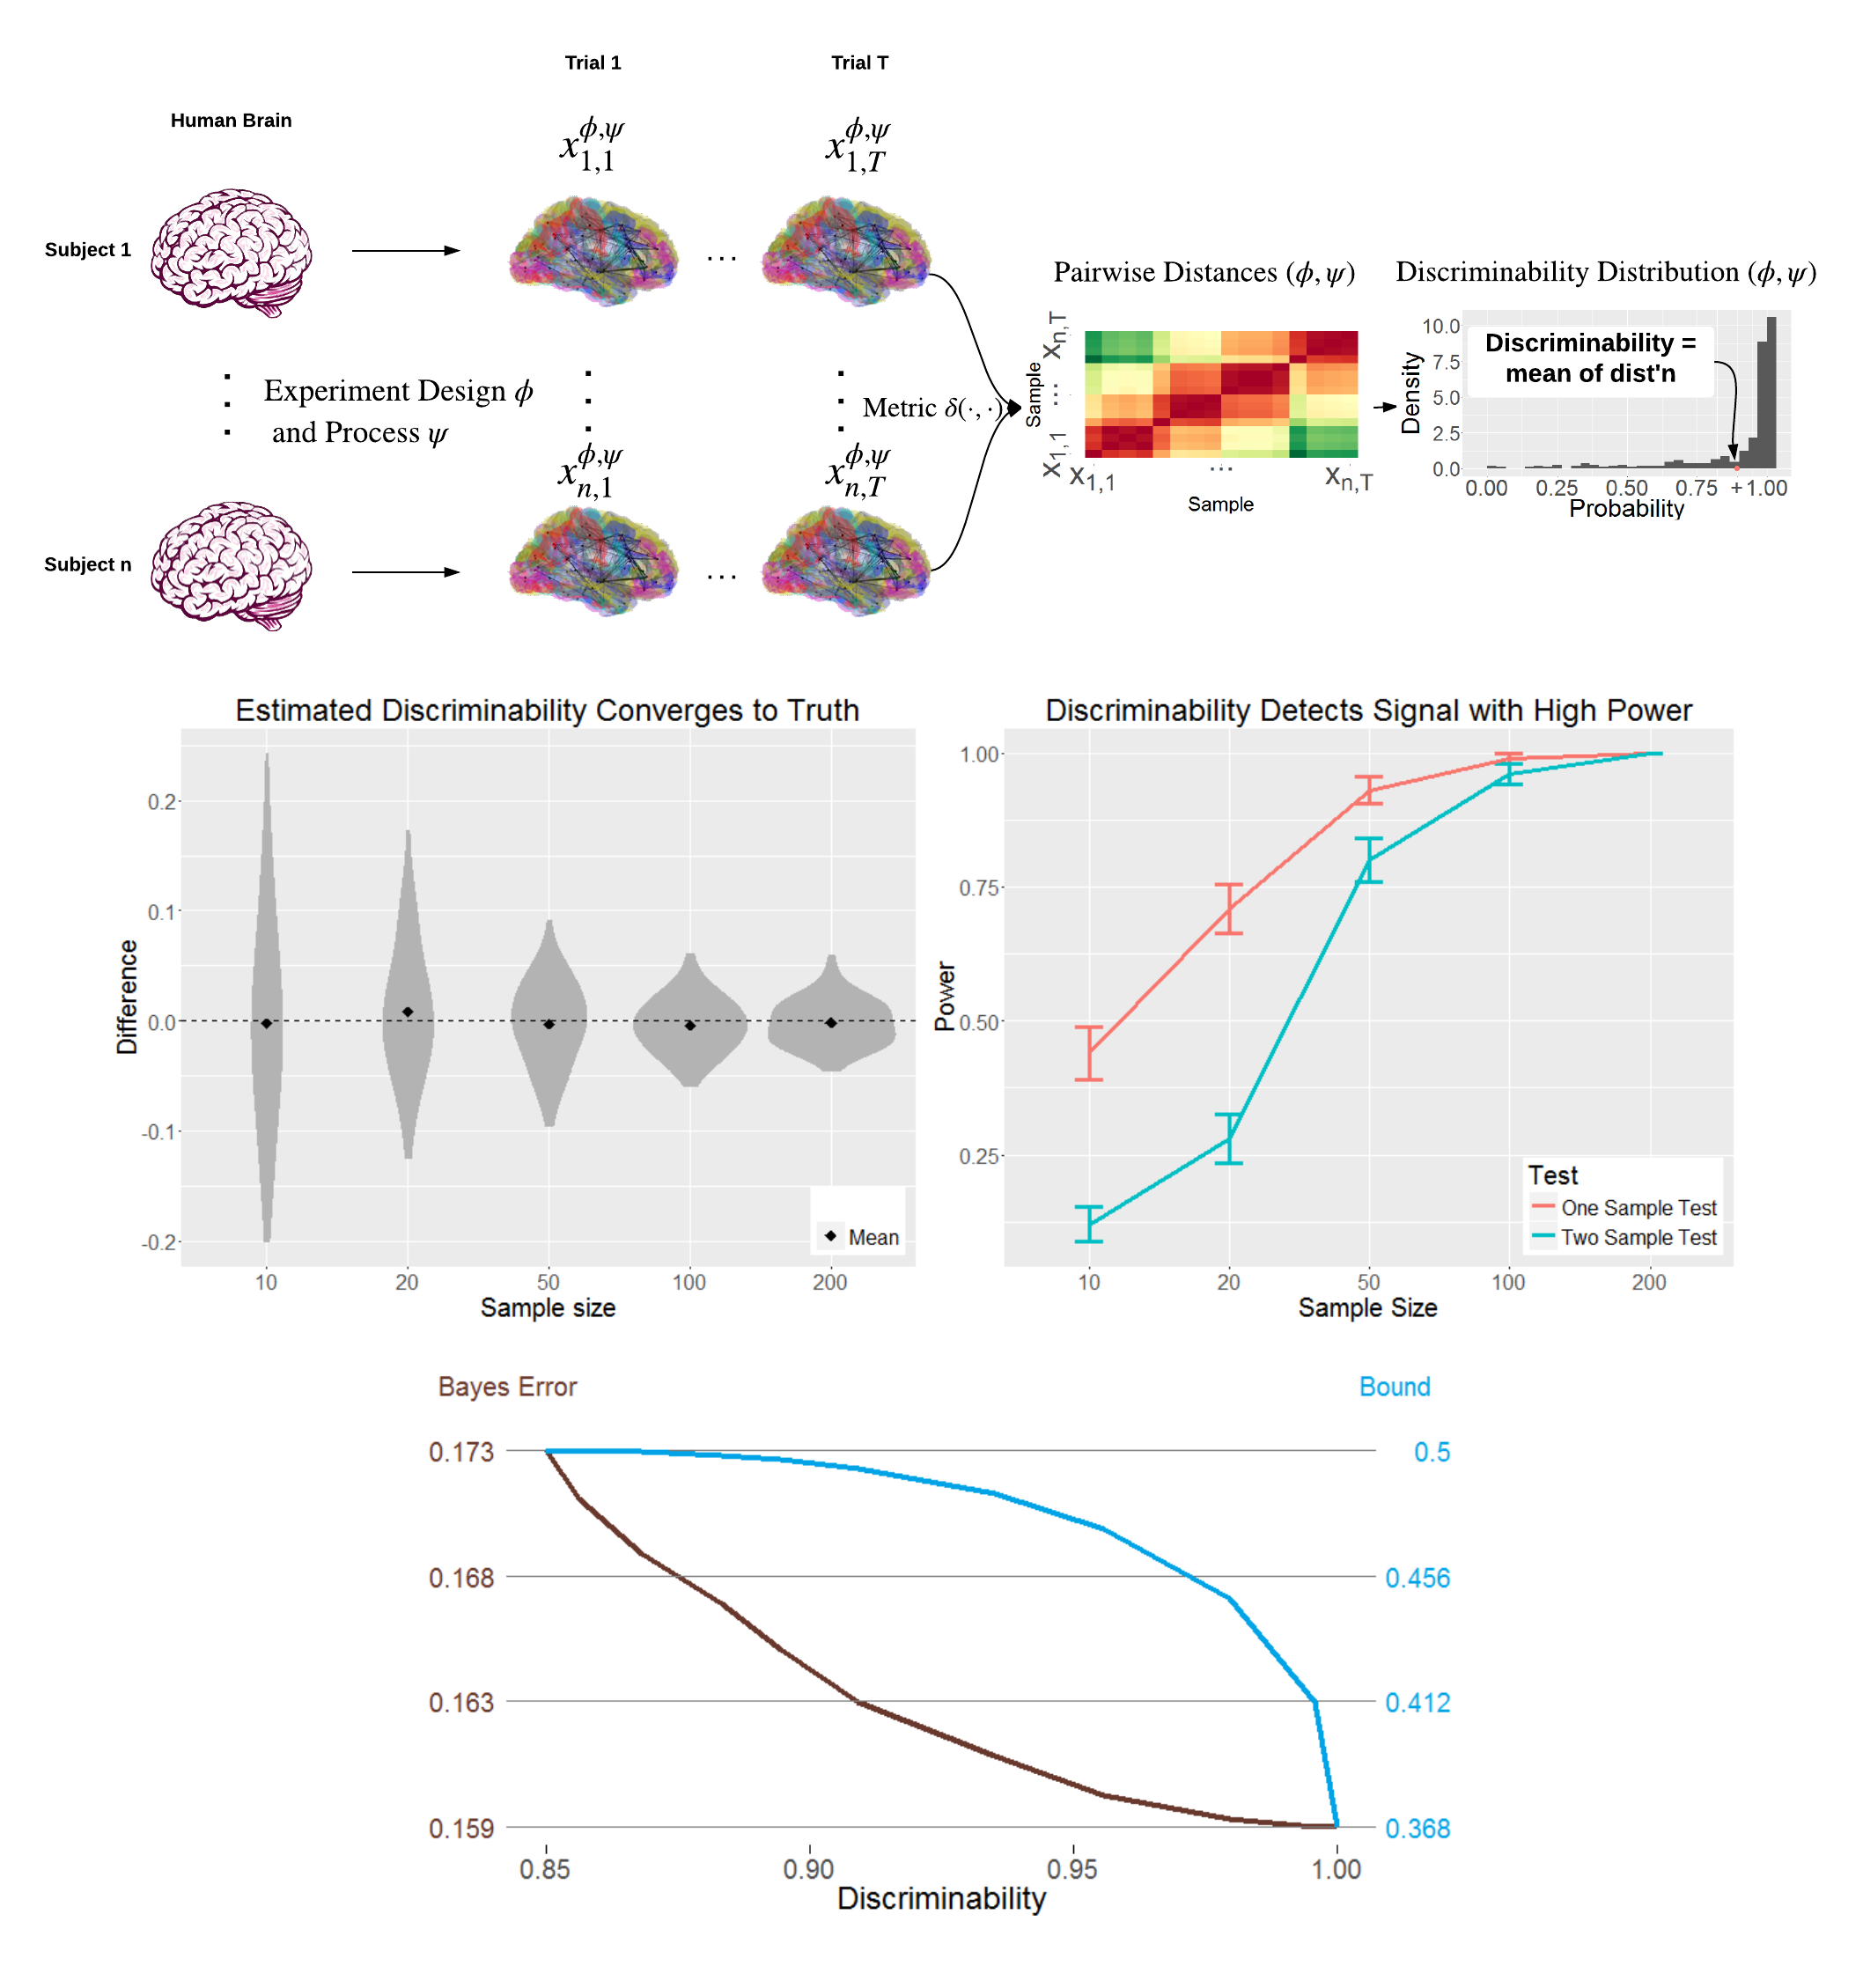
\includegraphics[width=\linewidth]{../Figs/flow_simu.png}
	\caption{{\bf Decision Making Through Discriminability Framework.} The top panel shows the decision framework of discriminability. Test-retest data set is collected under experiment design options $phi$ and processed by pipeline $\psi$. The pairwise distances of all measurements are computed using a metric $\delta(\cdot,\cdot)$. For each pair of measurements of the same subject, we estimate the probability of across subject distances being larger than the within subject distance. Discriminability is the mean of estimated probabilities. Select the option and pipeline with maximum discriminability. 
	\newline {\bf Convergence of $\hat{D}$.} Distribution of difference between discriminability estimates and truth is shown in the bottom left panel. The physical property and noise are generated from standard Gaussian distribution as described in the simulation section. The black dots indicate the mean over $100$ repeats. As the number of subjects increases, the sample discriminability converges to the true population discriminability.
	\newline {\bf Discriminability Test Power.} Test power of discriminability with varying sample size is shown in the bottom right panel. The physical property and noise are generated from standard Gaussian distribution as described in the simulation section. At level of $0.05$, the power is estimated based on $100$ repeats. The test power becomes close to $1$ with more than $50$ samples.}
	\label{fig:fc}
\end{figure}

\subsubsection{Estimating discriminability}
In real applications, distribution of $\bx_{i,t}$ may never known to us; hence, it is not possible to compute discriminability $D(\bpsi)$ or $D$ in short when there is no ambiguity in processing pipelines under consideration. However, samples $x_{i,t}$ are observed, and we can approximate true discriminability $D$ using an estimator $\hat{D}$ which is a function of observed samples. For each pair of observations $x_{i,t}$ and $x_{i,t'}$ from subject $i$, we first define
\[ \hat{D}_{i,t,t'} = \frac{\sum\limits_{i' \neq i}^{n} \sum\limits_{t''=1}^{s} \mathbb{I}\{\delta_{i,t,t'} \leq \delta_{i,i',t,t''} \} }{(n-1)s}\]
where $\mathbb{I}\{ \cdot \} $ is the indicator function, $n$ is the number of subjects, and $s$ denotes the number of observations per subject. $\hat{D}_{i,t,t'}$ is the faction of observations from other subjects farther away from $x_{i,t}$ than $x_{i,t'}$. It approximates the probability that distances from observations of other subjects to the $t^{th}$ observation of subject $i$ is larger than the distance between $t^{th}$ and $t'^{th}$ trial of subject $i$. Then, we define the discriminability estimator $\hat{D}$ to be the mean of $\hat{D}_{i,t,t'}$ averaged over all pairs of observations from same subjects.
\[ \hat{D} := \frac{\sum\limits_{i=1}^{n} \sum\limits_{t=1}^{s}  \sum\limits_{t' \neq t}^{s} \hat{D}_{i,t,t'}}{ns(s-1)} \]
$\hat{D}$ is the sample discriminability which approximates discriminability or population discriminability. The next two lemmas asserts that the discriminability estimator $\hat{D}$ is unbiased and converges to $D$ as the number of subjects $n$ goes to infinity \cite{bickel2015mathematical}.

\begin{lem}	
	$\hat{D}$ is an unbiased estimator of $D$, that is
	\[ \EE(\hat{D}) = D\]
	\label{lem:lem1}
\end{lem}

\begin{lem}	
	As $n \rightarrow \infty$, $\hat{D}$ converges to $D$ in probability, that is
	\[\hat{D} \overset{p}{\rightarrow} D \]
	\label{lem:lem2}
\end{lem}

\subsubsection{One Sample Testing Discriminability}
In applications, we sometimes are interested in whether there is any subject specific information in the data. In other words, we want to know whether $\bx_{i,t}$ is independent of $\bv_i$. Formally, it is equivalent to test the hypothesis that $\bx_{i,t}$ is independent of $\bv_i$. If we fail to reject the hypothesis, it implies the measurement $\bx_{i,t}$ reveals no information of true physical property $\bv_i$. As a consequence, $\bx_{i,t}$ is independent of any phenotype $\by_i$, and there is no hope in predicting $\by_i$ based on $\bx_{i,t}$. If this is the case, the researchers should consider collecting more data or processing data differently. Since $\bv_i$ is unobserved and $\by_i$ is unknown, a direct independence test is not applicable. We consider a test through discriminability. If measurements are independent of physical properties, $\bx_{i,t}$ and $\bx_{i',t'}$ should follow the same distribution. In this case, within subject distances should not differ across subject distances in distribution; therefore, discriminability should be $0.5$. Conversely, we have the following lemma.
\begin{lem}	
	Under additive noise model, disrcriminability is $0.5$ implies measurements are independent of physical property, that is 
	\[D=0.5 \Rightarrow \bx \perp \bv  .  \]
	\label{lem:lem3}
\end{lem}
An immediate consequence of the lemma is that we can test the null hypothesis that measurements $\bx_{i,t}$ are independent of any phenotype $\by_i$ through testing the hypothesis whether discriminability is $0.5$. Specifically, we reject the following null hypothesis when there is strong evidence suggesting that $D > 0.5$.
\[ H_0 \text{ : } \bx \perp \by \text{ ,and } H_A \text{ : } \bx \not\perp \by \]
We have two valid approaches to determine $D > 0.5$ through discriminability estimate $\hat{D}$. The first approach takes the advantage of the bound on variance of $\hat{D}$ which we derived in proving Lemma ~\ref{lem:lem2}. Specifically, we show that the variance of $\hat{D}$ is less than or equal to $1/n$. Based on Chebyshev's inequality, we can derive a 95 percent confidence interval $(\hat{D}-\frac{2\sqrt{5}}{\sqrt{n}},\hat{D}+\frac{2\sqrt{5}}{\sqrt{n}})$. If $0.5$ lies in the confidence interval, we do not reject the null hypothesis; otherwise, we reject the null hypothesis. This approach is computationally simple; however, generally has much smaller level and power due to the bound on variance is not tight. The second approach based on estimating a null distribution for $\hat{D}$ through permutation. In particular, we randomly permute subject labels for each trial and then estimate discriminability based on permuted labels. We repeat this procedure a large number of times and find the $95^{th}$ quantile of permuted discriminability estimates. If $\hat{D}$ is less than the $95^{th}$ quantile, we do not reject the null hypothesis; otherwise, we reject the null hypothesis. This approach has larger power, the only downside is that estimating discriminability for permuted samples takes sometime. In most applications, with less than a few hundred measurements, we recommend using the second approach. 

\subsubsection{Two Sample Testing Discriminability}
In many applications, we want to know whether one data processing pipeline $\bpsi_1$ yields more discriminable data set than another pipeline $\bpsi_2$. Based on the theory, by choosing the processing pipeline with larger discriminability, we can have a lower bound on Bayes prediction error. To achieve this, we consider testing the null hypothesis that two discriminabilities are equal.
\[H_0 \text{ : } D(\bpsi_1) = D(\bpsi_2) \text{ ,and }  H_A \text{ : } D(\bpsi_1) > D(\bpsi_2)\] 
However, $D(\bpsi_1)$ and $D(\bpsi_2)$ are not known to us, we have to decide based on estimators $\hat{D}(\bpsi_1)$ and $\hat{D}(\bpsi_2)$. We have two valid approaches to test this. The first approach takes the advantage of the bound on variance of $\hat{D}$ which we derived in proving Lemma ~\ref{lem:lem2}. Specifically, we show that the variance of discriminability estimate is bounded by $1/n$. Therefore, we can derive two confidence intervals centered at $\hat{D}(\bpsi_1)$ and $\hat{D}(\bpsi_2)$. Then, the null hypothesis is rejected if two confidence intervals does not overlap. Unfortunately, due to the fact that inequalities are not tight, this approach has very low power. For this method to work, the number of subjects $n$ usually needs to be larger than a thousand. It is impractical for most of the data set. The second approach estimates null distribution of $\hat{D}(\bpsi_1) - \hat{D}(\bpsi_2)$ through bootstrapping. We can bootstrap copies of the original data set and compute discriminability on bootstrapped data set to approximate the null distribution. Specifically, let $\hat{D}^{(i)}(\bpsi_j)$ denote the discriminability estimate for $i$th bootstrapped copy with data processed by pipeline $j$. If the null hypothesis is true, $\hat{D}(\bpsi_1) - \hat{D}(\bpsi_2)$ should have similar distribution as $\hat{D}^{(i)}(\bpsi_j)-\hat{D}^{(i')}(\bpsi_j)$. To bootstrap a copy of original data set, we need to make sure the copy have the same number of subjects and number of measurements per as the original data set. To bootstrap measurements for a subject, we first randomly choose two subjects from original data sets, and then take a random convex linear combination of measurements of these two subjects. We keep repeating this step until the bootstrapped data set has the same number of subjects as the original data set, and discriminability $\hat{D}^{(i)}(\bpsi_j)$ is estimated. To approximate the null distribution, a large number of bootstrapped discriminabilities are computed, and their pairwise differences $\hat{D}^{(i)}(\bpsi_j)-\hat{D}^{(i')}(\bpsi_j)$ are used to compute a p-value for $\hat{D}(\bpsi_1) - \hat{D}(\bpsi_2)$. We should notice that bootstrapped data tends to be less discriminable than the original data due to the fact bootstrapped subjects are closer to each other. However, only differences in bootstrapped discriminability are used. The algorithm \ref{alg:1} summarizes the steps to estimate p-value for testing $D(\bpsi_1) = D(\bpsi_2)$. 

\begin{algorithm}                      % enter the algorithm environment
	\caption{Test the null hypothesis $D(\bpsi_1) = D(\bpsi_2)$}          % give the algorithm a caption
	\label{alg:1}                           % and a label for \ref{} commands later in the document
	\begin{algorithmic}                    % enter the algorithmic environment
		\REQUIRE Data set, Pipeline $\bpsi_1$, Pipeline $\bpsi_2$
		\ENSURE Reject or do not reject the null hypothesis
		\STATE Process the data set with pipelines $\bpsi_1$ and $\bpsi_2$
		\STATE Compute $\hat{D}(\bpsi_1)$ and $\hat{D}(\bpsi_2)$
		\FOR{i in 1 through number of repeats} 
				\FOR{j in 1 through number of subjects} 
					\STATE Randomly select two subjects from data set 
					\STATE Linearly combine measurements of these subjects
				\ENDFOR
				\STATE Form two bootstrapped data sets processed by $\bpsi_1$ and $\bpsi_2$
				\STATE Compute $\hat{D}^{(i)}(\bpsi_1)$ and $\hat{D}^{(i)}(\bpsi_2)$
		\ENDFOR
		\STATE Compute pairwise differences $\hat{D}^{(i)}(\bpsi_1)-\hat{D}^{(i')}(\bpsi_1)$ and $\hat{D}^{(i)}(\bpsi_2)-\hat{D}^{(i')}(\bpsi_2)$
		\STATE Compute p-value which is the faction of times that $\hat{D}(\bpsi_1)-\hat{D}(\bpsi_2)>\hat{D}^{(i)}(\bpsi_j)-\hat{D}^{(i')}(\bpsi_j)$ 
		\STATE Reject the null hypothesis if p-value is less than $0.05$.
	\end{algorithmic}
\end{algorithm}

\subsection{Simulations}
\subsubsection{Convergence of discriminability estimator}
In Lemma \ref{lem:lem1} and  \ref{lem:lem2}, we claim discriminability $\hat{D}$ is unbiased and converges to  the true population discriminability in probability. We demonstrate these two lemmas through simulation. We consider a simple case that $g_{\bpsi}$ and $f_{\bphi}$ together introduce independent additive Gaussian noise $\epsilon$, that is
\begin{equation}
\bx_{i,t} =g_{\bpsi} \big(f_{\bphi} (\bv_i) \big) =\bv_{i} + \mb{\epsilon}_{i,t}
\end{equation}  
$\bv_{i}$ and $\mb{\epsilon}_{i,t}$ are both independent and identically distributed standard Gaussian random variable, that is 
\[\bv_i \overset{i.i.d.}{\sim} \mathbb{G}(0,1) \text{ and  }\mb{\epsilon}_{i,t} \overset{i.i.d.}{\sim} \mathbb{G}(0,1)\] 
In addition, $\bv_{i}$ and $\mb{\epsilon}_{i,t}$ are assumed to be independent. \\
For each subject, we sample one true physical property $v_i$ and two noises $\epsilon_{i,t}$ with $t\in\{1,2\}$. Then, two measurements are generated by $x_{i,t} = v_{i} + \epsilon_{i,t}$. We let the number of subjects $n$ vary from $10$ to $200$. For each value of $n$, we repeatedly generate data and compute discriminability $100$ times using Euclidean distance. It leaves us $100$ estimates of discriminability $\hat{D}$. With this data generation scheme, we can actually compute the population discriminability $D$ through numerical integration. It turns out to be $0.6150$. Subtracting $D$ from $100$ $\hat{D}$s, we can estimate the distribution of estimation error. The figure ~\ref{fig:simu1} shows the difference between $\hat{D}$ and $D$. We can see that the mean of difference is centered around 0 and  discriminabiity estimates $\hat{D}$ tends to converge to $D$ as the number of subject increases.

\begin{figure}[ht!]
	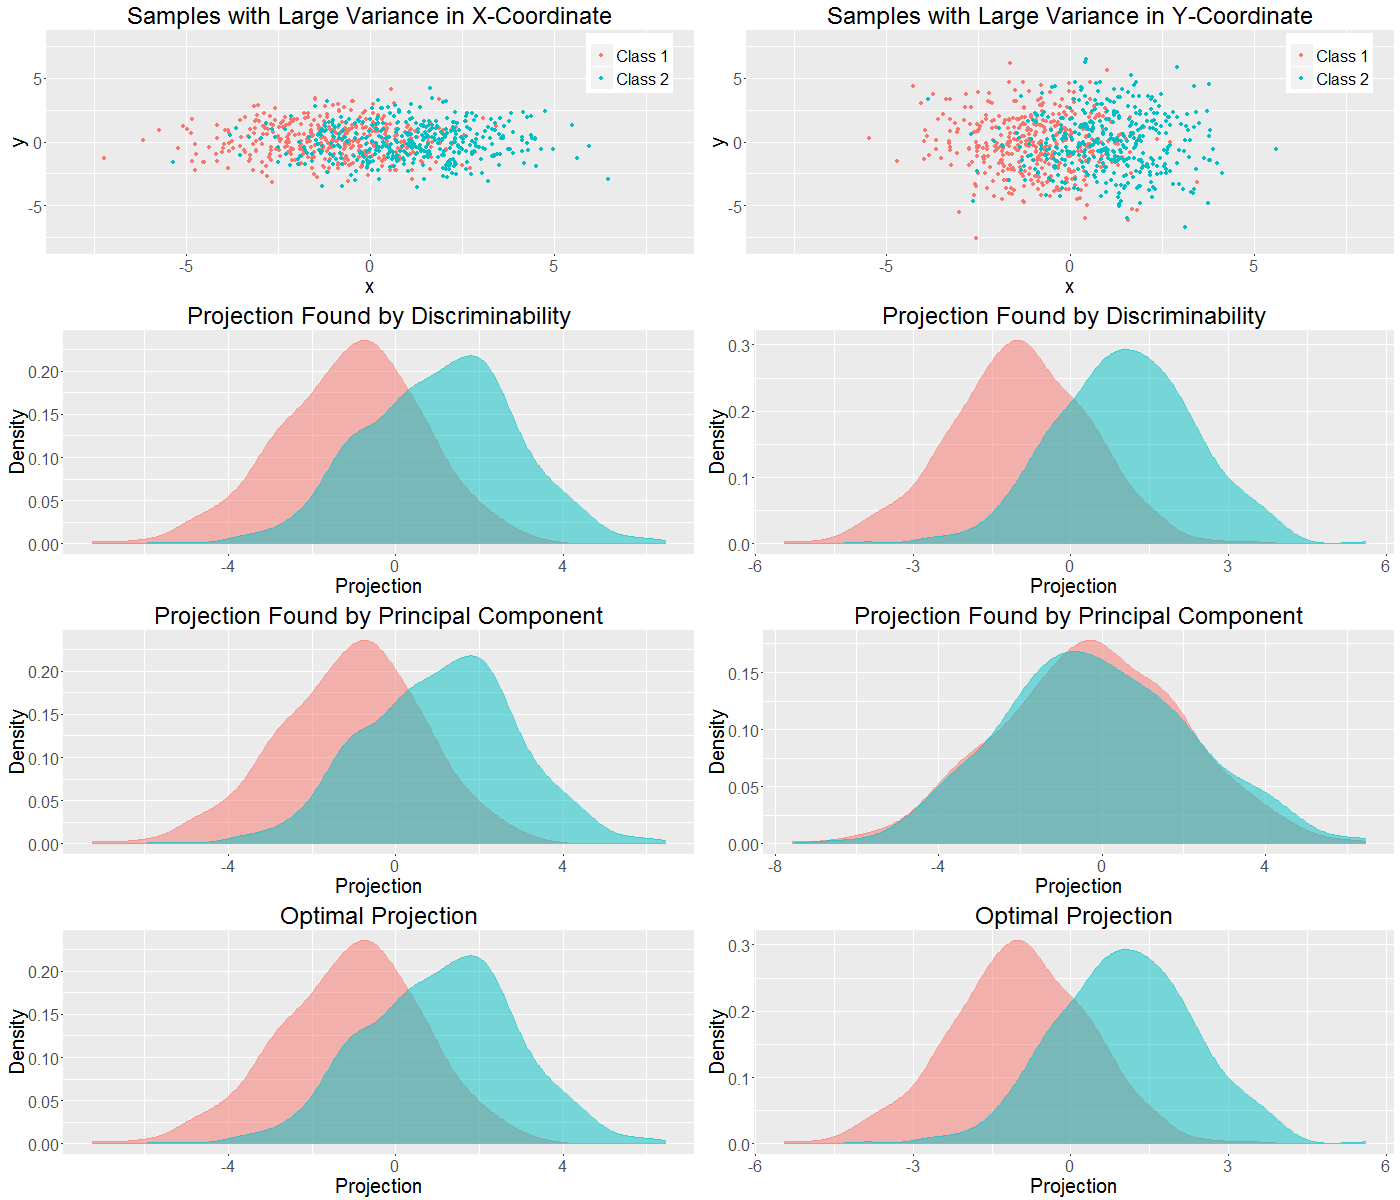
\includegraphics[width=\linewidth]{../Figs/simu2.png}
	\caption{{\bf Finding the Oprimal Projection.} Linear projections are computed using PCA and optimizing discriminability. Physical properties $\bv_i$ of $200$ subjects are sampled from 2-D two class conditional Gaussian distribution. $2$ measurements are sampled for each subject with additive Gaussian noise. Noise could have large variance in x-coordinate or y-coordinate. The details of generating data can be found in simulations section. The results for two cases are shown in two columns. Maximizing discriminability yields separated samples which have Bayes optimal classification error.}
	\label{fig:simu2}
\end{figure}




\subsubsection{Parameter selection through discriminability  }
In this simulation, we consider the task of projecting 2-dimensional observations linearly into 1-dimensional space. Like in the previous experiment, we assume independent additive noise. In addition to $\bx_{i,t}$, there is a binary class label $\by_{i}$ associated with subject $i$. The true physical property is Gaussian distributed conditioned on $\by_i$,
\[\bv_i|\by_i=1 \overset{i.i.d.}{\sim} \mathbb{G}(\begin{bmatrix}1\\0\end{bmatrix},\begin{bmatrix}1& 0\\0& 1\end{bmatrix}) \text{ and, } \bv_i|\by_i=0 \overset{i.i.d.}{\sim} \mathbb{G}(\begin{bmatrix}-1\\0\end{bmatrix},\begin{bmatrix}1& 0\\0& 1\end{bmatrix}) \]
We consider two cases for the distribution $\mb{\epsilon}_{i,t}$. The first case is that $\mb{\epsilon}_{i,t}$ has larger variance in the first coordinate; the other case is that $\mb{\epsilon}_{i,t}$ has larger variance in the second coordinate, that is
\[ \text{Case 1: } \mb{\epsilon}_{i,t} \sim \mathbb{G}(\begin{bmatrix}0\\0\end{bmatrix},\begin{bmatrix}2& 0\\0& 1\end{bmatrix}) \]
\[ \text{Case 2: } \mb{\epsilon}_{i,t} \sim \mathbb{G}(\begin{bmatrix}0\\0\end{bmatrix},\begin{bmatrix}1& 0\\0& 4\end{bmatrix}) \]
The noise is assumed to be independent of $\bv_i$ and $\by_i$. The figure ~\ref{fig:simu2} shows the scatter plot of measurements. Under this generation scheme, the class signal only exists in the first coordinate. Therefore, the optimal linear projection should only keep the first coordinate. \\
We sample $200$ subjects with $v_i$ from each class conditional distribution. Furthermore, $2$ measurements are sampled for each subject. We use both discriminability and principal component analysis (PCA) \cite{jolliffe2002principal} to find the optimal linear projection. After finding the projection, we estimate two class conditional distribution through a kernel density estimator \cite{silverman1986density}. The results of two cases are provided in two columns of figure ~\ref{fig:simu2}. In the first case, both methods find the optimal linear projection which separates two classes. However, in the second case only discriminability recovers the optimal projection. PCA finds linear projection with little class signal.




\subsection{Connectome Processing Applications}

\subsubsection{Optimal discriminability yields optimal predictive accuracy}
In this experiment, we are going to investigate the thresholding step in processing resting state functional magnetic resonance imaging (fMRI). In fMRI processing, time series is first extracted for each region of interest (ROI) of brain \cite{strother2006evaluating}. Then, a pairwise connectivity matrix is estimated through computing absolute Pearson correlation \cite{liang2012effects}. To remove noise and obtain a binary graph, the pairwise connectivity matrix needs to be thresholded by a value which lies in $[0,1]$ \cite{hampson2002detection,van2010exploring}. We would like to find the optimal value for the threshold. In addition to neuroimages, demographic information and five neuro factors \cite{costa1992revised} are also collected from each subject. We also want to find the threshold which leads to graphs with the best prediction performance.  

HCP100 data set is used in this experiment \cite{van2012human}. It contains data from $461$ subjects with $4$ measurements per subject. We let the threshold vary from 0 to 1. For each value of the threshold, binary graphs is constructed by thresholding correlations. Then, the discriminability is computed with Euclidean distance. In addition, sex, age and the neuro factors are predicted using k-nearest neighbor \cite{vapnik1998statistical}. For comparison, another reliability statistics, namely image intraclass correlation coefficient is also computed which generalizes intraclass correlation coefficient for high dimensional observations \cite{shou2013quantifying}. The discriminability, I2C2, and prediction errors versus the values of threshold are shown in figure ~\ref{fig:hcp}. The threshold which maximizes discriminability is close to the thresholds yielding smallest predicting errors for three covariates. 



\begin{figure}[H]
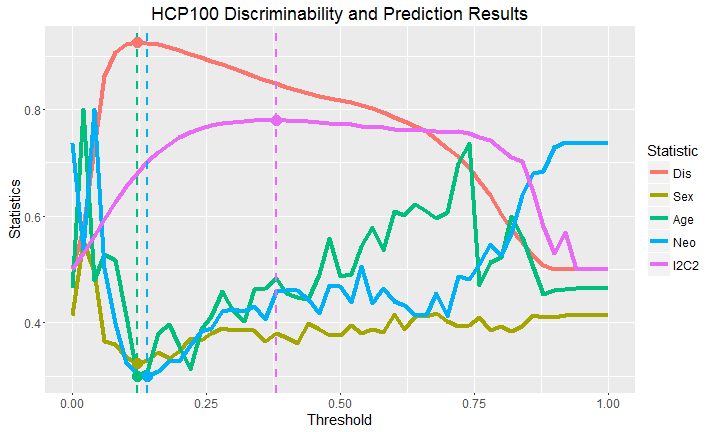
\includegraphics[width=\linewidth]{../Figs/HCP_100.png}
\caption{{\bf Optimizing discriminability yields optimal prediction accuracy for multiple covariates.} HCP100 is used to investigate optimal threshold to convert correlation graphs into binary graphs. Curves are scaled to have similar value range. For each statistic, the optimal threshold and value pair is indicated by a circle on the curve. The threshold maximizing discriminability is close to the optimal thresholds for predicting three covariates. }
\label{fig:hcp}
\end{figure}

\subsubsection{fMRI processing pipelines}
In this experiment, we are going to investigate the pre-processing options in acquiring resting state fMRI graphs \cite{huettel2004functional}. There have been a lot of steps proposed for pre-processing connectomes in the last decade. Here, we study a subset of them. In particular, we are interested in options include atlas \cite{mai2015atlas}, anatomical registration \cite{klein2009evaluation}, temporal filtering \cite{smith1999investigation}, motion correction \cite{power2012spurious} and nuisance signal regression \cite{fox2009global}. We want to find the optimal pre-processing pipeline and the best decision for each option. We are going to index each pipeline by five letters which is explained in the table below.   
\begin{center}
	\begin{tabular}{ |c|c| } 
		\hline
		Option & Letter  \\ \hline
		Atlas & C for CC200, H for HOX, A for AAL, D for DES \cite{craddock2012whole,desikan2006automated} \\ \hline
		Anatomical Registration & F for FSL, A for ANTS \cite{andersson2007non,avants2009advanced}\\ \hline
		Temporal Filtering & F for frequency filtering, X for not  \cite{smith1999investigation}\\ \hline
		Motion Correction & S for scrubbing, X for not  \cite{power2012spurious} \\ \hline
		Nuisance Signal Regression & G for global signal regression , X for not \cite{fox2009global} \\ \hline
	\end{tabular}
\end{center}
As an example, the best pipeline found is CFXSG which means the data is pre-processed using CC200 atlas, registered with FSL, no frequency filtering, with scrubbing and with global signal regression. There are $4$ possible choices for atlas and $2$ possible choices for other options. This leaves us $64$ different combinations of options. We select $13$ test-retest fMRI data sets with the number of measurements ranging from $50$ to $300$. These data sets are pre-processed by the $64$ pipelines through the configurable pipeline for the analysis of connectomes (c-pac) \cite{sikka2014towards}. We also consider an extra rank conversion step which proves to be helpful in boosting discriminability. Rank conversion transforms a weighted undirected graph into a graph with rank weights. Specifically, in the previous experiment all edge weights are absolute correlations which lie in $[0,1]$. In rank conversion step, for each edge in a graph, its weight $w$ is replaced by the rank of $w$ among all edge weights. If we denote a graph by a node set and an edge weight set pair $(V,E)$ with $E=\{w_{i,j}\}$, rank conversion is a function
\[(V,E) \rightarrow (V,E') \text{ , where } E'= \{\text{rank}(w_{i,j})\} \]
The rank conversion is designed to improve signal to noise ratio by removing background noise. We carry out this step on the $13$ data sets pre-processed by $64$ pipelines and compare the difference in discriminability with rank conversion and without rank conversion. The figure ~\ref{fig:pipes} shows the discriminability of rank fMRI graphs and the discriminability of raw fMRI graphs are provided in appendix. It turns out that the rank conversion does help improving mean discriminability in all pipelines. When global signal regression is not performed, rank conversion significantly boosts discriminability.

There is notable variation in discriminability. The mean discriminability across $13$ data sets can vary from $0.77$ to $1.00$. CFXSG turns out to be the best pipeline with maximum mean discriminability. Furthermore, we carried out a multi-factor analysis of variance test to study each option \cite{hair2009multivariate}. Specifically, we fix decision for all options except one, and attempts to see whether there is significant difference in discriminability. It turns out that FSL, no frequency filtering, no scrubbing, global signal regression and rank conversion is better than their alternatives in terms of mean discriminability. However, fsl and no scrubbing is not statistical significantly better at level $0.05$. No frequency filtering, global signal regression and rank conversion is better than their alternatives at level $0.001$. Figure ~\ref{fig:decs} shows the distribution of paired difference in discriminability.
 
\newpage
\begin{figure}[H]
	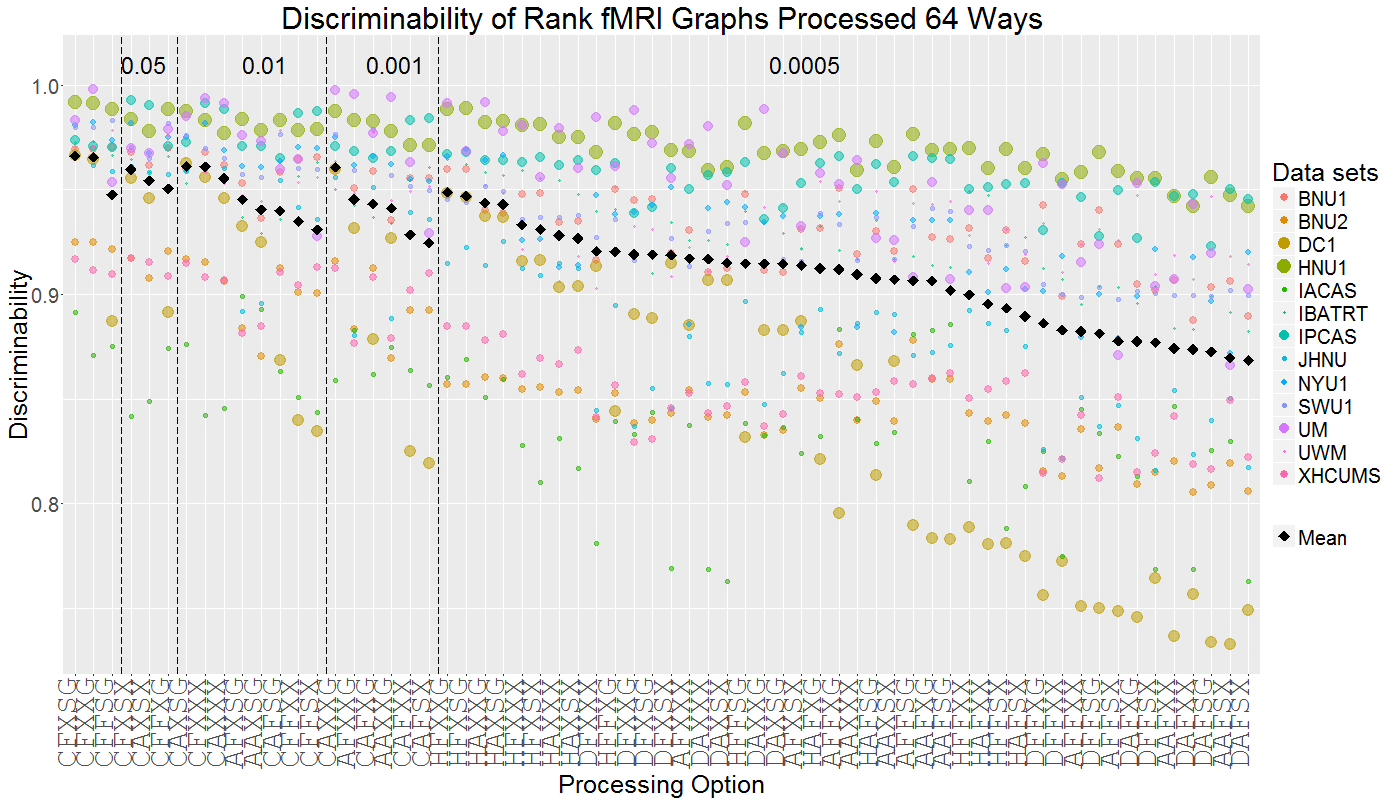
\includegraphics[width=\linewidth]{../Figs/fmri_rank_pv.png}
	\caption{{\bf Discriminability of rank fmri graphs from 13 data sets processed 64 ways.}  Discriminability of BNU1, BNU2, DC1,HNU1, IACAS, IBATRT, IPCAS, JHNU, NYU1, SWU1, UM, UWM and XHCUMS pre-processed by 64 pipelines are computed and shown in the top panel. Color of each dot indicates data set and size indicates the number of measurements in data set. The black square indicates the weighted mean discriminability across 13 data sets. The pipelines are first grouped by p-values when comparing to pipeline CFXXG using Wilcoxon signed-rank test. Within each group, the pipelines are ordered by the mean discriminability. CFXSG pipeline has the best mean discriminability across data sets.}
	\label{fig:pipes}
\end{figure}

\begin{figure}[H]
	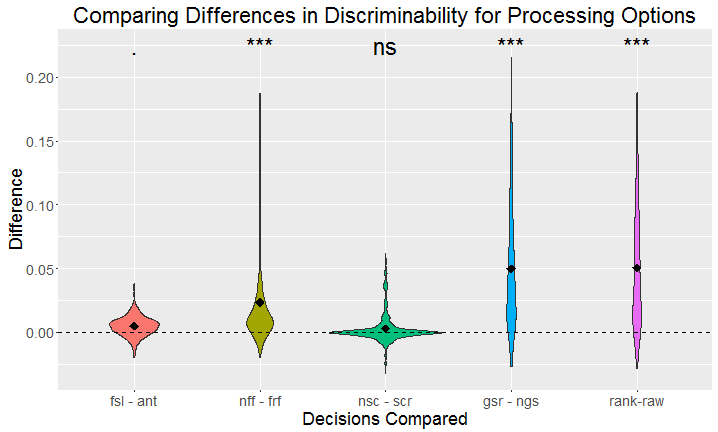
\includegraphics[width=\linewidth]{../Figs/mri_decs.png}
	\caption{{ \bf Paired difference in discriminability of pre-processing options.} Difference in discriminability for each option is compared by fixing the other options and data set. The symbols at top indicates the significance. No frequency filtering, global signal regression and rank conversion are statistical significantly better than their alternatives at level $0.001$. Fsl and no scrubbing are not significantly better. }
	\label{fig:decs}
\end{figure}



\subsubsection{DTI experiment design}
In this experiment, we consider the experiment design of collecting DTI data. In particular, we are interested the effect of b-value and number of directions on discriminability \cite{westin2002processing}. We pick four data sets with different b-value and number of directions and compute discriminability. The result is show in the right panel of figure ~\ref{fig:comb_dti}. We can see they have comparable discriminability. Given four data sets, we cannot conclude the optimal value for the parameters. It would be ideal if we could carry out a more controlled study with more data.

\begin{figure}[H]
	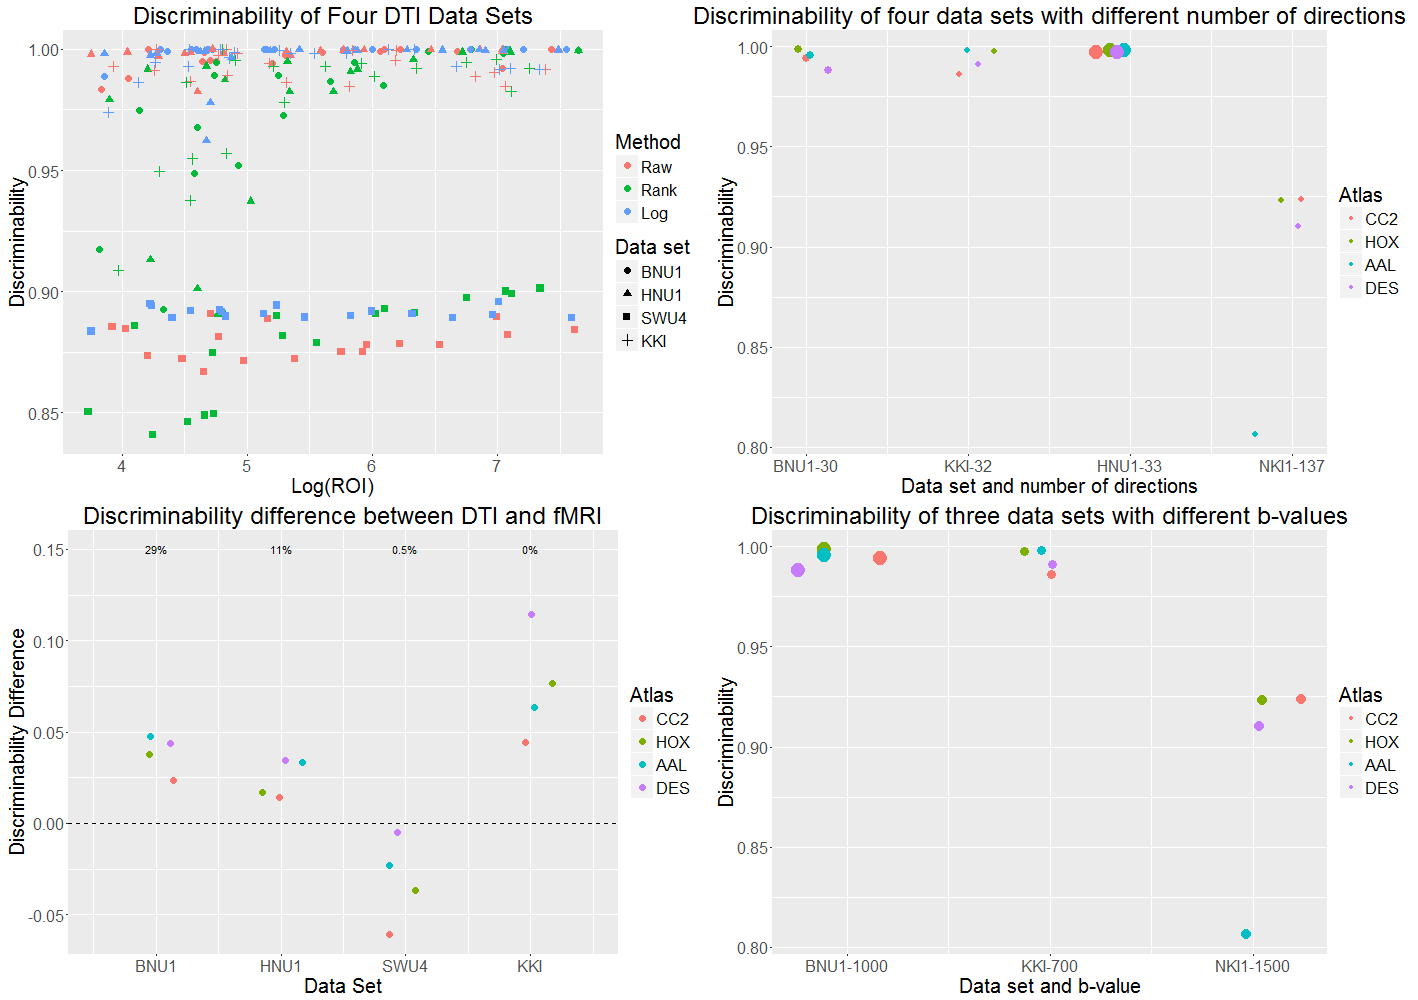
\includegraphics[width=\linewidth]{../Figs/comb_dti.png}
	\caption{{ \bf Discriminability of DTI data sets.} The top left plot shows the discriminability of SWU4 registered with 15 atlases are computed and shown in the top panel. Raw, rank and log edges weights are considered. Discriminability of DTI and fMRI graphs are compared for BNU1, HNU1, SWU4 and KKI data set. The results are shown in the bottom left panel. The number at the top indicates the percentage of outliers in DTI data sets. After removing outliers, DTI data sets tend to be more discriminable than fMRI data sets. The right column shows the result of discriminability of different data sets with different b-value and number of directions.}
	\label{fig:comb_dti}
\end{figure}


\subsubsection{DTI processing pipelines}
In this experiment, we consider the processing of diffusion tensor imaging (DTI) \cite{westin2002processing}. In particular, we are interested in finding the optimal number of ROI, and the optimal approach to process edge weights. BNU1, HNU1, SWU4 and KKI data sets are used in this experiment. We process four DTI data sets using 15 atlases with the number of ROI ranging from $48$ to $1875$ \cite{mori2005mri}. For edge weights, we consider three options. First, raw edge weights are used which are fiber counts. Furthermore, we consider two alternatives: log weights and rank weights as discussed in the previous experiment. Top left panel of figure ~\ref{fig:comb_dti} shows the results. We see discriminability is basically stable across different atlases when raw and log edge weights are used. When using the rank weights, discriminability is low when the number of ROI is small. For three out of four data sets, the discriminability is very close to $1$. As a consequence, we cannot find any statistical relationship between the number of ROI and discriminability.




\subsubsection{fMRI vs. DTI}
In this experiment, we want to compare discriminanility of fMRI and DTI data sets. Four data sets with both fMRI and DTI images are selected for the comparison. In processing fMRI data sets, the most dicriminable pipeline (*FXXG) is used. In processing DTI data sets, we use the raw edge weights. Some DTI measurements fail to pass the processing pipeline or have a dubious small number of edges. In this case, these measurements are labeled as outliers and removed from discriminability calculation. The result is shown in the bottom left panel of figure ~\ref{fig:comb_dti}. Our conclusion is that DTI data sets after outlier removal have comparable discriminability as fMRI data sets. Actually, DTI measurements are better than fMRI in three out of four data sets. 



\section{Discussion}

\para{Summary} We propose a non-parametric statistics of discriminability which is define to be the probability that within subject distance is smaller than across subject distance.  We prove discriminability bounds Bayes prediction error. An estimator is designed to estimate the discriminability based on test-retest data set. We show the estimator is unbiased and converges to the discriminability asymptotically. Furthermore, we developed one sample and two sample tests for discriminability, which can be used to detect signal in real data set and compare discriminability of different processing pipelines. We apply the discriminability framework under various setups in neuroimaging processing. We find the best processing pipeline for fMRI pre-processing and look into options in DTI processing. Furthermore, fMRI and DTI are shown to have comparable discriminability.



\para{Next Steps} From theoretical point of view, most of our theories require the noise to be additive and independent of subjects. The effects of subject specific noise on discriminability are left uninvestigated. As for applications, more experiments should be carried out to analyze processing options. In particular, we could investigate processing of DTI more thoroughly given more data sets. Also, the effect of the number of ROI on discriminability is still not determined. Second, metrics other than Euclidean distance could be studied. Third, a testing procedure could be developed for comparing discriminability of multiple data sets.



\section{Appendix}


% \input{intro}
% \input{simulations}
% \input{flow}
% \input{setting}
% \input{logic}
% \input{main}
% \input{setup}
% \input{gRAICAR}



\appendix
\begin{figure}[H]
	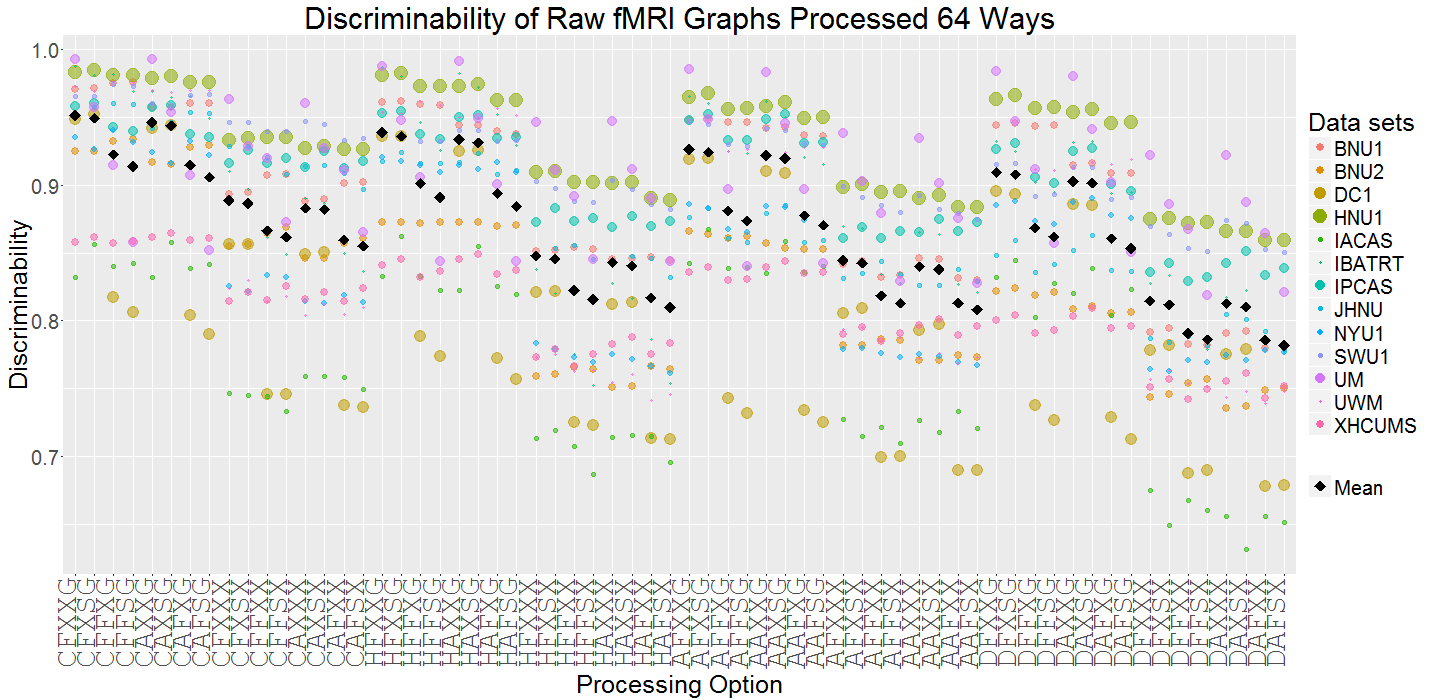
\includegraphics[width=\linewidth]{../Figs/fmri_raw.png}
	\caption{{\bf Discriminability of raw fmri graphs from 13 data sets processed 64 ways.}  Discriminability of BNU1, BNU2, DC1, HNU1, IACAS, IBATRT, IPCAS, JHNU, NYU1, SWU1, UM, UWM and XHCUMS pre-processed by 64 pipelines are computed and shown in the top panel. Color of each dot indicates data set and size indicates the number of measurements in data set. The black square indicates the weighted mean discriminability across 13 data sets. CFXXG pipeline has the best mean discriminability across data sets.}
	\label{fig:raw}
\end{figure}
\begin{proof}[Proof of Theorem 1]
	Consider the additive noise setting, that is $\bx_{i,t}=\bv_{i} + \mb{\epsilon}_{i,t}$,  
	\begin{eqnarray*}
		& &\PP(\delta_{i,t,t'} \leq \delta_{i,i',t,t''}) \\
		&=&\PP(\|\bx_{i,t}-\bx_{i,t'}\|<\|\bx_{i,t}-\bx_{i',t''}\|) \\
		&=&\PP(\|\mb{\epsilon}_{i,t}-\mb{\epsilon}_{i,t'}\| < \|\bv_{i}+\mb{\epsilon}_{i,t}-\bv_{i'}-\mb{\epsilon}_{i',t''}\|) \\
		&\leq&\PP(\|\mb{\epsilon}_{i,t}-\mb{\epsilon}_{i,t'}\| < \|\bv_{i}-\bv_{i'}\| + \|\mb{\epsilon}_{i,t}-\mb{\epsilon}_{i',t''}\|) \\
		&=& \PP(\|\mb{\epsilon}_{i,t}-\mb{\epsilon}_{i,t'}\|-\|\mb{\epsilon}_{i,t}-\mb{\epsilon}_{i',t''}\|< \|\bv_{i}-\bv_{i'}\|) \\
		&=& \frac{1}{2}\PP(\|\mb{\epsilon}_{i,t}-\mb{\epsilon}_{i,t'}\|-\|\mb{\epsilon}_{i,t}-\mb{\epsilon}_{i',t''}\|< \|\bv_{i}-\bv_{i'}\||\|\mb{\epsilon}_{i,t}-\mb{\epsilon}_{i,t'}\|-\|\mb{\epsilon}_{i,t}-\mb{\epsilon}_{i',t''}\|<0) + \\ 
		& &\frac{1}{2}\PP(\|\mb{\epsilon}_{i,t}-\mb{\epsilon}_{i,t'}\|-\|\mb{\epsilon}_{i,t}-\mb{\epsilon}_{i',t''}\|< \|\bv_{i}-\bv_{i'}\||\|\mb{\epsilon}_{i,t}-\mb{\epsilon}_{i,t'}\|-\|\mb{\epsilon}_{i,t}-\mb{\epsilon}_{i',t''}\|>0) \\
		&=&\frac{1}{2} + \frac{1}{2}\PP(\|\mb{\epsilon}_{i,t}-\mb{\epsilon}_{i,t'}\|-\|\mb{\epsilon}_{i,t}-\mb{\epsilon}_{i',t''}\|< \|\bv_{i}-\bv_{i'}\||\|\mb{\epsilon}_{i,t}-\mb{\epsilon}_{i,t'}\|-\|\mb{\epsilon}_{i,t}-\mb{\epsilon}_{i',t''}\|>0) \\
		&=& \frac{1}{2} + \frac{1}{2}\PP(\big| \|\mb{\epsilon}_{i,t}-\mb{\epsilon}_{i,t'}\|-\|\mb{\epsilon}_{i,t}-\mb{\epsilon}_{i',t''}\| \big|< \|\bv_{i}-\bv_{i'}\|)\\
		&=& 1 - \frac{1}{2} \PP(\big| \|\mb{\epsilon}_{i,t}-\mb{\epsilon}_{i,t'}\|-\|\mb{\epsilon}_{i,t}-\mb{\epsilon}_{i',t''}\| \big|> \|\bv_{i}-\bv_{i'}\|)\\
	\end{eqnarray*}
	To bound the probability above, we bound the $\|\bv_{i}-\bv_{i'}\|$ and $\big| \|\mb{\epsilon}_{i,t}-\mb{\epsilon}_{i,t'}\|-\|\mb{\epsilon}_{i,t}-\mb{\epsilon}_{i',t''}\| \big|$ separately. We start with the first term.
	\begin{eqnarray*}
		& &\EE(\|\bv_{i}-\bv_{i'}\|^2) \\
		&=&\EE(\bv_{i}^T \bv_{i}+\bv_{i'}^T\bv_{i'} -2\bv_{i}^T \bv_{i'}) \\
		&=&2\sigma_2^2
	\end{eqnarray*}
	Here, $\sigma_2^2$ is the trace of covariance matrix of $\bv_{i}$. We can apply Markov's Inequality, 
	\[、\PP(\|\bv_{i}-\bv_{i'}\| < t) \geq 1 - \frac{2 \sigma_2^2}{t^2} \]
	Let $\sigma_1^2$ denote the trace of covariance matrix of ${\epsilon}_{i,t}$, and let $a$ and $b$ be two constants satisfy
	\[\EE(\big| \|\mb{\epsilon}_{i,t}-\mb{\epsilon}_{i,t'}\|-\|\mb{\epsilon}_{i,t}-\mb{\epsilon}_{i',t''}\| \big|^2) \geq a^2 \sigma_1^2\]
	\[\frac{\EE^2(\big| \|\mb{\epsilon}_{i,t}-\mb{\epsilon}_{i,t'}\|-\|\mb{\epsilon}_{i,t}-\mb{\epsilon}_{i',t''}\| \big|^2)}{\EE(\big| \|\mb{\epsilon}_{i,t}-\mb{\epsilon}_{i,t'}\|-\|\mb{\epsilon}_{i,t}-\mb{\epsilon}_{i',t''}\| \big|)^4} \geq b \]
	Then, we can apply Paley-Zygmund Inequality \cite{paley1932some},
	\[\PP(\big| \|\mb{\epsilon}_{i,t}-\mb{\epsilon}_{i,t'}\|-\|\mb{\epsilon}_{i,t}-\mb{\epsilon}_{i',t''}\| \big|^2 > t^2 ) \geq b(1-\frac{t^2}{a^2 \sigma_1^2})^2 \]
	Understand the fact that $\bv$s and $\mb{\epsilon}$s are independent, we can combine the two inequalities and get a bound on $\PP(\delta_{i,t,t'} \leq \delta_{i,i',t,t''})$.
	\begin{eqnarray*}
		& &\PP(\delta_{i,t,t'} \leq \delta_{i,i',t,t''}) \\
		&=&\PP(\|\bx_{i,t}-\bx_{i,t'}\|<\|\bx_{i,t}-\bx_{i',t''}\|)  \\
		&\leq& 1 - \frac{1}{2} \PP(\big| \|\mb{\epsilon}_{i,t}-\mb{\epsilon}_{i,t'}\|-\|\mb{\epsilon}_{i,t}-\mb{\epsilon}_{i',t''}\| \big|> \|\bv_{i}-\bv_{i'}\|) \\
		&\leq& 1 - \frac{1}{2}\PP(\big| \|\mb{\epsilon}_{i,t}-\mb{\epsilon}_{i,t'}\|-\|\mb{\epsilon}_{i,t}-\mb{\epsilon}_{i',t''}\| \big|^2 > t^2 )P(\|\bv_{i}-\bv_{i'}\|^2 < t^2) \\
		&\leq& 1- \frac{1}{2}b(1-\frac{t^2}{a^2 \sigma_1^2})^2(1 - \frac{2 \sigma_2^2}{t^2})
	\end{eqnarray*}
	Assume $a^2 \sigma_1^2 \geq 2 \sigma_2^2$ and set $t^2=\sqrt{2} a \sigma_1 \sigma_2$,
	\begin{eqnarray*}
		\PP(\|\bx_{i,t}-\bx_{i,t'}\|<\|\bx_{i,t}-\bx_{i',t''}\|) \leq  1- \frac{1}{2}b(1 - \frac{\sqrt{2} \sigma_2}{a\sigma_1})^3
	\end{eqnarray*}
	By definition, $D=\PP(\|\bx_{i,t}-\bx_{i,t'}\|<\|\bx_{i,t}-\bx_{i',t''}\|)$, we can have a bound on $\frac{ \sigma_2}{\sigma_1}$.
	\begin{equation}
	\frac{ \sigma_2}{\sigma_1} \geq\frac{a}{\sqrt{2}} (1-(\frac{2-2D}{b})^{1/3} )
	\end{equation}	
	To obtain a bound on Bayes error, we apply Devijver and Kittler's result \cite{devijver1982pattern},
	\[L \leq \frac{2\pi_0\pi_1}{1+\pi_0\pi_1\Delta\mu^T\Sigma^{-1}\Delta\mu}\]
	Here, $\pi_0$ and $\pi_1$ are prior probabilities for two classes. $\Delta\mu$ is the difference between means of two classes. Since $\mb{\epsilon}$ is assumed to be independent of $\bx$ and $\by$,
	\[\Delta\mu= \EE(\bx|\by=0)-\EE(\bx|\by=1)=\EE(\bv|\by=0)-\EE(\bv|\by=1)\]
	$\Sigma$ is the weighted covariance matrix of $\bx$,
	\begin{eqnarray*}
		\Sigma &=& \pi_0\text{Var}(\bx|\by=0)+\pi_1\text{Var}(\bx|\by=1)\\
		&=& \pi_0\text{Var}(\bv|\by=0)+\pi_1\text{Var}(\bv|\by=1)+\text{Var}(\mb{\epsilon}) \\ 
	\end{eqnarray*}
	If we further assume $\text{Var}(\mb{\epsilon}) = \lambda \Sigma'$ where the trace of $\Sigma$ is $1$, then equation 6 implies $\lambda\leq\lambda_*$, where
	\[\lambda_*=\frac{\sqrt{2}\sigma_2}{a(1-(\frac{2-2D}{b})^{1/3} )}\]
	Hence, 	$\Sigma \leq \Sigma_*$ where
	\begin{eqnarray*}
		\Sigma_*&=& \pi_0\text{Var}(\bv|\by=0)+\pi_1\text{Var}(\bv|\by=1)+\lambda^*\Sigma'
	\end{eqnarray*}
	Therefore, $\Sigma^{-1} \geq \Sigma_*^{-1}$, and we have
	\begin{eqnarray*}
		L &\leq& \frac{2\pi_0\pi_1}{1+\pi_0\pi_1\Delta\mu^T\Sigma^{-1}\Delta\mu} \\
		&\leq& \frac{2\pi_0\pi_1}{1+\pi_0\pi_1\Delta\mu^T\Sigma_*^{-1}\Delta\mu}
	\end{eqnarray*}
\end{proof}



\begin{proof}[Proof of Lemma 1]
	By definition of $\hat{D}$,
	\[\hat{D}= \frac{\sum\limits_{i=1}^{n} \sum\limits_{t=1}^{s}  \sum\limits_{t'\neq t}^{s} \hat{D}_{i,t,t'}}{ns(s-1)}\]
	The expectation of $\hat{D}_{i,t,t'}$ is actually $D$,
	\begin{eqnarray*}  
		& &\EE(\hat{D}_{i,t,t'}) \\
		&=&\frac{\sum\limits_{i' \neq i}^{n} \sum\limits_{t''=1}^{s} 		    	 \EE(\mathbb{I}\{\delta_{i,t,t'} \leq \delta_{i,i',t,t''} \}) }{(n-1)s} \\
		&=&\frac{\sum\limits_{i' \neq i}^{n} \sum\limits_{t''=1}^{s} 
		     	\PP[\delta_{i,t,t'} \leq \delta_{i,i',t,t''}]}{(n-1)s} \\
		&=& \frac{\sum\limits_{i' \neq i}^{n} \sum\limits_{t''=1}^{s} 
			D}{(n-1)s} \\
		&=& D
	\end{eqnarray*}
	Therefore, we have
	\begin{eqnarray*}
		& &\EE(\hat{D})\\
		&=&\frac{\sum\limits_{i=1}^{n} \sum\limits_{t=1}^{s}  \sum\limits_{t'\neq t}^{s} \EE(\hat{D}_{i,t,t'})}{ns(s-1)} \\
		&=&\frac{\sum\limits_{i=1}^{n} \sum\limits_{t=1}^{s}  \sum\limits_{t'\neq t}^{s} D}{ns(s-1)} \\
		&=& D
	\end{eqnarray*}
	This concludes that $\hat{D}$ is an unbiased estimator of discriminability $D$.
\end{proof}

\begin{proof}[Proof of Lemma 2]
	By definition of $\hat{D}$,
	\begin{eqnarray*}  
		\hat{D} &=&\frac{\sum\limits_{i=1}^{n} \sum\limits_{t=1}^{s}  \sum\limits_{t'\neq t}^{s} \hat{D}_{i,t,t'}}{ns(s-1)}\\
		&=& \frac{\sum\limits_{i=1}^{n} \sum\limits_{t=1}^{s}  \sum\limits_{t'\neq t}^{s}\sum\limits_{i' \neq i}^{n} \sum\limits_{t''=1}^{s} \mathbb{I}\{\delta_{i,t,t'} \leq \delta_{i,i',t,t''} \} }{ns(s-1)(n-1)s}\\
		&=& \frac{\sum\limits_{i,i',t,t',t''} \mathbb{I}\{\delta_{i,t,t'} \leq \delta_{i,i',t,t''} \}  }{ns(s-1)(n-1)s}
	\end{eqnarray*}
	In the last step, we simplify the sum, but keep in mind that $i\neq i'$ and $t \neq t'$. We show in the previous lemma that $\EE(\hat{D})=D$. To demonstrate that $\hat{D}$ converges to $D$ in probability, it is suffice to show that $\text{Var}(\hat{D}) \rightarrow 0$. Since then, by Chebyshev's inequality,
	\[\PP[|\hat{D}-D| \geq \epsilon] \leq \frac{\text{Var}(\hat{D})}{\epsilon^2} \rightarrow 0\]
	If we expand the variance of $R$, 
	\[\text{Var}(\hat{D})= \frac{\sum\limits_{i,i',t,t',t''} \sum\limits_{j,j',r,r',r''} \text{Cov}(\mathbb{I}\{\delta_{i,t,t'} \leq \delta_{i,i',t,t''} \},\mathbb{I}\{\delta_{j,r,r'} \leq \delta_{j,j',r,r',r''} \})}{(ns(s-1)(n-1)s)^2} \]
	There are $(ns(s-1)(n-1)s)^2$ covariance terms in the sum of nominator; however, most of them are actually $0$. $\mathbb{I}\{\delta_{i,t,t'} \leq \delta_{i,i',t,t''}$ is a function of $\bx_{i,t}$, $\bx_{i,t'}$ and $\bx_{i',t''}$; therefore, is independent of any observations of subjects other than $i$ and $i'$. This implies $\mathbb{I}\{\delta_{i,t,t'} \leq \delta_{i,i',t,t''} \}$ is independent of $\mathbb{I}\{\delta_{j,r,r'} \leq \delta_{j,j',r,r',r''} \}$ as long as $\{i,i'\} \cap \{j,j'\} = \emptyset$. As a consqeunce, there are $(4n-6)(s(s-1)s)=ns(s-1)(n-1)s-(n-2)s(s-1)(n-3)s$ combinations of $j,j',r,r',r''$ such that covariance between $\mathbb{I}\{\delta_{i,t,t'} \leq \delta_{i,i',t,t''} \}$ and $\mathbb{I}\{\delta_{j,r,r'} \leq \delta_{j,j',r,r',r''} \}$ maybe non-zero. Furthermore, the covariance must be less $\frac{1}{4}$ due to the fact that they are indicator random variables. Therefore, we have 
	\begin{eqnarray*} 
		\text{Var}(\hat{D})&=& \frac{\sum\limits_{i,i',t,t',t''} \sum\limits_{j,j',r,r',r''} \text{Cov}(\mathbb{I}\{\delta_{i,t,t'} \leq \delta_{i,i',t,t''} \},\mathbb{I}\{\delta_{j,r,r'} \leq \delta_{j,j',r,r',r''} \})}{(ns(s-1)(n-1)s)^2} \\
		&\leq& \frac{\sum\limits_{i,i',t,t',t''}  (4n-6)(s(s-1)s)}{4(ns(s-1)(n-1)s)^2} \\
		&=& \frac{ (4n-6)(s(s-1)s)}{4ns(s-1)(n-1)s} \\
		&=& \frac{4n-6}{4n(n-1)} \\
		&\leq& \frac{1}{n}  \\
		&\rightarrow& 0 \text{ , as $n\rightarrow \infty$} 
	\end{eqnarray*}
	As discussed before, this concludes that $\hat{D}$ converges to $D$ in probability. 
\end{proof}


\begin{proof}[Proof of Lemma 3]
	Consider the additive noise setting, that is $\bx_{i,t}=\lambda \bv_{i} + \mb{\epsilon}_{i,t}$. We further assume  $\bv_{i}$ and $\mb{\epsilon}_{i,t}$ have continuous distributions. We will show that $D=0.5$ implies $\lambda = 0$, hence $\bx_{i,t} = \mb{\epsilon}_{i,t}$ which is independent of physical property $\bv_{i}$ and any phenotype $\by_{i}$. First, we rewrite the definition of discriminability.
	\begin{eqnarray*}
		& &\PP(\delta_{i,t,t'} \leq \delta_{i,i',t,t''}) \\
		&=&\PP(\|\bx_{i,t}-\bx_{i,t'}\|<\|\bx_{i,t}-\bx_{i',t''}\|) \\
		&=&\PP(\|\mb{\epsilon}_{i,t}-\mb{\epsilon}_{i,t'}\| < \|\lambda \bv_{i}+\mb{\epsilon}_{i,t}-\lambda \bv_{i'} - \mb{\epsilon}_{i',t''}\|) \\
		&=& \EE (\PP(\|\mb{\epsilon}_{i,t}-\mb{\epsilon}_{i,t'}\| < \|v+\mb{\epsilon}_{i,t} - \mb{\epsilon}_{i',t''}\|)|\|\lambda \bv_{i} - \lambda \bv_{i'}=v)
	\end{eqnarray*}
	We will to show for any $v \neq 0$,   \[\PP(\|\mb{\epsilon}_{i,t}-\mb{\epsilon}_{i,t'}\| < \|v+\mb{\epsilon}_{i,t} - \mb{\epsilon}_{i',t''}\|) > 0.5\]
	Therefore, $D=0.5$ implies $\lambda \bv_{i} - \lambda \bv_{i'}= 0$. Since $\bv_{i}$ is not constant, we have $\lambda = 0$. Due to $\mb{\epsilon}$ being i.i.d., we have 
	\[\PP(\|\mb{\epsilon}_{i,t}-\mb{\epsilon}_{i,t'}\| < \|v+\mb{\epsilon}_{i,t} - \mb{\epsilon}_{i',t''}\|) =  \PP(\|\mb{\epsilon}_{i,t}-\mb{\epsilon}_{i',t''}\| < \|v+\mb{\epsilon}_{i,t} - \mb{\epsilon}_{i,t'}\|)\]
	Consider the sum of these two probabilities, we will show it is greater than $1$. Let $A$ and $B$ denote the set where the conditions of two events hold respectively.
	\begin{eqnarray*}
			& &\PP(\|\mb{\epsilon}_{i,t}-\mb{\epsilon}_{i,t'}\| < \|v+\mb{\epsilon}_{i,t} - \mb{\epsilon}_{i',t''}\|) +  \PP(\|\mb{\epsilon}_{i,t}-\mb{\epsilon}_{i',t''}\| < \|v+\mb{\epsilon}_{i,t} - \mb{\epsilon}_{i,t'}\|)\\
			&=&\PP(A) + \PP(B) \\
			&=& 2\PP(A \cap B ) + \PP(A \cap B^c ) + \PP(B \cap A^c ) \\
			&=& 1+\PP(A \cap B )- \PP(A^c \cap B^c )
	\end{eqnarray*}
	We first notice that $A^c \cap B^c$ implies $\|-\mb{\epsilon}_{i,t}+\mb{\epsilon}_{i,t'}\| < \|v-\mb{\epsilon}_{i,t} + \mb{\epsilon}_{i',t''}\|$ and $\|-\mb{\epsilon}_{i,t}+\mb{\epsilon}_{i',t''}\| < \|v-\mb{\epsilon}_{i,t} + \mb{\epsilon}_{i,t'}\|$. In addition, due to symmetry
	\[\PP(A \cap B ) = 
	\PP(\|-\mb{\epsilon}_{i,t}+\mb{\epsilon}_{i,t'}\| < \|v-\mb{\epsilon}_{i,t} + \mb{\epsilon}_{i',t''}\| \text{ ,and } \|-\mb{\epsilon}_{i,t}+\mb{\epsilon}_{i',t''}\| < \|v-\mb{\epsilon}_{i,t} + \mb{\epsilon}_{i,t'}\|) .\] 
	As a consequence, we have $ \PP(A^c \cap B^c) < \PP(A \cap B ) $. This shows 
	\[\PP(\|\mb{\epsilon}_{i,t}-\mb{\epsilon}_{i,t'}\| < \|v+\mb{\epsilon}_{i,t} - \mb{\epsilon}_{i',t''}\|) +  \PP(\|\mb{\epsilon}_{i,t}-\mb{\epsilon}_{i',t''}\| < \|v+\mb{\epsilon}_{i,t} - \mb{\epsilon}_{i,t'}\|) > 1 .\]
	Hence,
	\[\PP(\|\mb{\epsilon}_{i,t}-\mb{\epsilon}_{i,t'}\| < \|v+\mb{\epsilon}_{i,t} - \mb{\epsilon}_{i',t''}\|) > 0.5\]
	As discussed previously, this concludes the proof for the lemma.
\end{proof}



\begin{table}
% latex table generated in R 3.2.2 by xtable 1.8-2 package
%
\scalebox{0.6}{ 
\begin{tabular}{rrrrrrrrrrrrrrr}
	\hline
	& BNU1 & BNU2 & DC1 & HNU1 & IACAS & IBATRT & IPCAS & JHNU & NYU1 & SWU1 & UM & UWM & XHCUMS & Mean \\ 
	\hline
	AAFXG & 0.927449 & 0.859286 & 0.783674 & 0.968958 & 0.883002 & 0.913690 & 0.965035 & 0.872126 & 0.935463 & 0.940903 & 0.953237 & 0.942917 & 0.860072 & 0.906543 \\ 
	CAFXG & 0.958776 & 0.912551 & 0.878391 & 0.982635 & 0.861788 & 0.936756 & 0.965118 & 0.951149 & 0.965926 & 0.978910 & 0.976981 & 0.977500 & 0.908134 & 0.943180 \\ 
	DAFXG & 0.904592 & 0.809388 & 0.745649 & 0.955347 & 0.813185 & 0.895833 & 0.926615 & 0.831034 & 0.899259 & 0.901645 & 0.952915 & 0.947083 & 0.815091 & 0.877574 \\ 
	HAFXG & 0.931633 & 0.850408 & 0.821087 & 0.972802 & 0.832156 & 0.932292 & 0.962496 & 0.892816 & 0.937037 & 0.938578 & 0.957631 & 0.954167 & 0.852645 & 0.912378 \\ 
	AAFXX & 0.906735 & 0.820204 & 0.736838 & 0.946837 & 0.846388 & 0.883929 & 0.946720 & 0.854310 & 0.873241 & 0.899595 & 0.906958 & 0.918750 & 0.841630 & 0.874231 \\ 
	CAFXX & 0.955306 & 0.892143 & 0.824902 & 0.971091 & 0.863632 & 0.954613 & 0.983267 & 0.939080 & 0.954907 & 0.951387 & 0.963114 & 0.949167 & 0.901775 & 0.928410 \\ 
	DAFXX & 0.887449 & 0.805306 & 0.756704 & 0.941923 & 0.768578 & 0.883185 & 0.947552 & 0.823563 & 0.917685 & 0.899536 & 0.942756 & 0.907083 & 0.818967 & 0.873794 \\ 
	HAFXX & 0.917143 & 0.839184 & 0.780752 & 0.960229 & 0.829744 & 0.947173 & 0.951257 & 0.885920 & 0.901111 & 0.921220 & 0.940256 & 0.915000 & 0.854547 & 0.895432 \\ 
	AAFSG & 0.926122 & 0.859286 & 0.783174 & 0.969225 & 0.885593 & 0.912946 & 0.964327 & 0.875575 & 0.935185 & 0.939825 & 0.907079 & 0.944167 & 0.862428 & 0.901947 \\ 
	CAFSG & 0.958061 & 0.912551 & 0.868578 & 0.982884 & 0.863346 & 0.936012 & 0.965035 & 0.954598 & 0.963519 & 0.976601 & 0.959889 & 0.978333 & 0.910417 & 0.940007 \\ 
	DAFSG & 0.903469 & 0.808878 & 0.733706 & 0.955676 & 0.825443 & 0.898810 & 0.922952 & 0.839655 & 0.896759 & 0.898874 & 0.919536 & 0.946667 & 0.816286 & 0.872551 \\ 
	HAFSG & 0.930306 & 0.848776 & 0.813679 & 0.973060 & 0.828661 & 0.935268 & 0.962163 & 0.891379 & 0.938796 & 0.936730 & 0.926832 & 0.949167 & 0.853243 & 0.907630 \\ 
	AAFSX & 0.906020 & 0.819490 & 0.732669 & 0.947456 & 0.829847 & 0.891369 & 0.950175 & 0.850575 & 0.872037 & 0.902058 & 0.866202 & 0.918333 & 0.849167 & 0.869789 \\ 
	CAFSX & 0.955408 & 0.892551 & 0.819409 & 0.971189 & 0.856785 & 0.960565 & 0.983808 & 0.935632 & 0.954167 & 0.949848 & 0.929090 & 0.951667 & 0.910236 & 0.924556 \\ 
	DAFSX & 0.889388 & 0.805918 & 0.749095 & 0.942073 & 0.762786 & 0.882440 & 0.945346 & 0.817529 & 0.919907 & 0.899693 & 0.902241 & 0.914167 & 0.822174 & 0.868462 \\ 
	HAFSX & 0.915612 & 0.838469 & 0.774974 & 0.960006 & 0.808320 & 0.927083 & 0.952756 & 0.875000 & 0.902593 & 0.920602 & 0.903249 & 0.919167 & 0.862482 & 0.889531 \\ 
	AAXXG & 0.935306 & 0.869592 & 0.926577 & 0.977625 & 0.874870 & 0.933780 & 0.968115 & 0.888506 & 0.962130 & 0.956745 & 0.994195 & 0.945000 & 0.878822 & 0.941187 \\ 
	CAXXG & 0.959490 & 0.915918 & 0.959734 & 0.987269 & 0.858750 & 0.950149 & 0.970779 & 0.955747 & 0.975093 & 0.976601 & 0.997299 & 0.963333 & 0.912428 & 0.960729 \\ 
	DAXXG & 0.911224 & 0.832857 & 0.882894 & 0.967266 & 0.832765 & 0.933780 & 0.936022 & 0.847414 & 0.934167 & 0.914255 & 0.988148 & 0.941667 & 0.836902 & 0.914707 \\ 
	HAXXG & 0.939898 & 0.860306 & 0.937136 & 0.982195 & 0.851007 & 0.958333 & 0.963786 & 0.913793 & 0.963796 & 0.951663 & 0.991897 & 0.952083 & 0.877808 & 0.943688 \\ 
	AAXXX & 0.919184 & 0.840000 & 0.866043 & 0.958981 & 0.840203 & 0.916667 & 0.950175 & 0.886207 & 0.884167 & 0.915994 & 0.963920 & 0.916667 & 0.851014 & 0.909469 \\ 
	CAXXX & 0.961429 & 0.906224 & 0.945712 & 0.976868 & 0.845372 & 0.956845 & 0.988137 & 0.960057 & 0.968889 & 0.964761 & 0.990970 & 0.952917 & 0.906612 & 0.955380 \\ 
	DAXXX & 0.910714 & 0.841327 & 0.906894 & 0.959308 & 0.768497 & 0.925595 & 0.956960 & 0.857471 & 0.940926 & 0.930265 & 0.980045 & 0.910833 & 0.843351 & 0.916880 \\ 
	HAXXX & 0.934184 & 0.853265 & 0.903516 & 0.974729 & 0.831239 & 0.954613 & 0.961705 & 0.914943 & 0.912870 & 0.936609 & 0.979400 & 0.906250 & 0.866431 & 0.928232 \\ 
	AAXSG & 0.936327 & 0.870408 & 0.924621 & 0.978401 & 0.892683 & 0.929315 & 0.970529 & 0.895690 & 0.960833 & 0.955668 & 0.973111 & 0.944167 & 0.884819 & 0.940364 \\ 
	CAXSG & 0.959898 & 0.916939 & 0.962326 & 0.987526 & 0.876065 & 0.953125 & 0.972361 & 0.958621 & 0.974722 & 0.975985 & 0.984762 & 0.962083 & 0.914891 & 0.961132 \\ 
	DAXSG & 0.910714 & 0.834898 & 0.882727 & 0.968451 & 0.836466 & 0.929315 & 0.941059 & 0.862069 & 0.937222 & 0.916718 & 0.967185 & 0.942500 & 0.842826 & 0.914656 \\ 
	HAXSG & 0.938469 & 0.859796 & 0.936799 & 0.982765 & 0.859188 & 0.956845 & 0.963745 & 0.925287 & 0.966481 & 0.949200 & 0.977747 & 0.948333 & 0.880996 & 0.943027 \\ 
	AAXSX & 0.920408 & 0.839388 & 0.868104 & 0.960410 & 0.834040 & 0.916667 & 0.953588 & 0.890517 & 0.881944 & 0.916610 & 0.925905 & 0.915833 & 0.858514 & 0.906926 \\ 
	CAXSX & 0.961633 & 0.907653 & 0.945716 & 0.977725 & 0.848962 & 0.958333 & 0.990301 & 0.958333 & 0.967500 & 0.964756 & 0.967105 & 0.956250 & 0.915109 & 0.954224 \\ 
	DAXSX & 0.912449 & 0.842143 & 0.906845 & 0.960479 & 0.763131 & 0.924107 & 0.958167 & 0.856897 & 0.943889 & 0.933805 & 0.951826 & 0.918333 & 0.846721 & 0.914974 \\ 
	HAXSX & 0.934796 & 0.854082 & 0.903895 & 0.975124 & 0.816855 & 0.947917 & 0.963828 & 0.912644 & 0.913704 & 0.937686 & 0.960050 & 0.917917 & 0.873152 & 0.926798 \\ 
	AFFXG & 0.950816 & 0.876122 & 0.795589 & 0.975918 & 0.883351 & 0.921131 & 0.965743 & 0.871839 & 0.938056 & 0.933357 & 0.952611 & 0.944167 & 0.852156 & 0.911937 \\ 
	CFFXG & 0.969898 & 0.920612 & 0.891382 & 0.988116 & 0.874132 & 0.965774 & 0.970613 & 0.957184 & 0.974907 & 0.981681 & 0.978916 & 0.975833 & 0.908424 & 0.950509 \\ 
	DFFXG & 0.942551 & 0.815612 & 0.756078 & 0.966950 & 0.825183 & 0.912202 & 0.930528 & 0.825862 & 0.901204 & 0.904711 & 0.962460 & 0.933750 & 0.814366 & 0.886296 \\ 
	HFFXG & 0.950306 & 0.852959 & 0.844117 & 0.981547 & 0.839326 & 0.940476 & 0.962746 & 0.894540 & 0.937963 & 0.935653 & 0.961155 & 0.951250 & 0.856667 & 0.920298 \\ 
	AFFXX & 0.923878 & 0.835510 & 0.751169 & 0.958355 & 0.844876 & 0.895089 & 0.946470 & 0.850862 & 0.879630 & 0.898507 & 0.915506 & 0.923750 & 0.842065 & 0.882388 \\ 
	CFFXX & 0.964388 & 0.901020 & 0.840061 & 0.978351 & 0.851011 & 0.956101 & 0.986347 & 0.941379 & 0.970278 & 0.960013 & 0.964438 & 0.953333 & 0.904203 & 0.934933 \\ 
	DFFXX & 0.898980 & 0.812959 & 0.772361 & 0.954986 & 0.775143 & 0.906994 & 0.953130 & 0.821839 & 0.918056 & 0.900009 & 0.952413 & 0.910417 & 0.821250 & 0.882955 \\ 
	HFFXX & 0.931429 & 0.843265 & 0.788678 & 0.969664 & 0.810602 & 0.949405 & 0.950008 & 0.892241 & 0.910463 & 0.922743 & 0.940309 & 0.928333 & 0.850272 & 0.899819 \\ 
	AFFSG & 0.950306 & 0.878061 & 0.789844 & 0.976540 & 0.881127 & 0.918155 & 0.965826 & 0.870977 & 0.935093 & 0.932280 & 0.908228 & 0.943333 & 0.856938 & 0.906584 \\ 
	CFFSG & 0.970000 & 0.921531 & 0.887307 & 0.988175 & 0.875197 & 0.966518 & 0.970280 & 0.958908 & 0.973333 & 0.983220 & 0.953521 & 0.978333 & 0.909656 & 0.947562 \\ 
	DFFSG & 0.940306 & 0.817041 & 0.750175 & 0.967727 & 0.833682 & 0.904018 & 0.927905 & 0.837069 & 0.899815 & 0.903171 & 0.923813 & 0.931250 & 0.811938 & 0.881276 \\ 
	HFFSG & 0.947959 & 0.853367 & 0.831813 & 0.981808 & 0.838350 & 0.939732 & 0.963079 & 0.896552 & 0.941389 & 0.934267 & 0.924960 & 0.949167 & 0.857989 & 0.914707 \\ 
	AFFSX & 0.923878 & 0.836327 & 0.748567 & 0.958796 & 0.822476 & 0.903274 & 0.949467 & 0.846839 & 0.878981 & 0.897427 & 0.871044 & 0.925833 & 0.851014 & 0.877746 \\ 
	CFFSX & 0.965408 & 0.900612 & 0.834690 & 0.978636 & 0.843672 & 0.962798 & 0.987304 & 0.935920 & 0.969907 & 0.959705 & 0.927571 & 0.955833 & 0.912862 & 0.930896 \\ 
	DFFSX & 0.901939 & 0.815204 & 0.764450 & 0.955244 & 0.768609 & 0.904018 & 0.953546 & 0.816092 & 0.921667 & 0.900619 & 0.903679 & 0.909583 & 0.824293 & 0.876907 \\ 
	HFFSX & 0.930510 & 0.842245 & 0.781240 & 0.969452 & 0.788431 & 0.923363 & 0.952423 & 0.882759 & 0.911759 & 0.923356 & 0.902650 & 0.930833 & 0.858442 & 0.893537 \\ 
	AFXXG & 0.950408 & 0.883163 & 0.931645 & 0.983162 & 0.883020 & 0.942708 & 0.968115 & 0.880460 & 0.961389 & 0.959370 & 0.995491 & 0.948333 & 0.876667 & 0.945379 \\ 
	CFXXG & 0.969082 & 0.925000 & 0.964223 & 0.991333 & 0.870641 & 0.973214 & 0.970529 & 0.961494 & 0.982037 & 0.979834 & 0.997983 & 0.970833 & 0.911558 & 0.965581 \\ 
	DFXXG & 0.945000 & 0.838367 & 0.890495 & 0.976575 & 0.833195 & 0.918899 & 0.938728 & 0.837069 & 0.939352 & 0.916256 & 0.987935 & 0.932500 & 0.829130 & 0.919107 \\ 
	HFXXG & 0.959490 & 0.856939 & 0.948355 & 0.988527 & 0.860303 & 0.964286 & 0.966866 & 0.914655 & 0.966111 & 0.945197 & 0.991337 & 0.946667 & 0.884692 & 0.948842 \\ 
	AFXXX & 0.930612 & 0.854286 & 0.885344 & 0.968144 & 0.837410 & 0.925595 & 0.950175 & 0.879885 & 0.885648 & 0.913356 & 0.971717 & 0.922500 & 0.852572 & 0.917045 \\ 
	CFXXX & 0.967857 & 0.915510 & 0.955905 & 0.983235 & 0.842025 & 0.960565 & 0.991009 & 0.959483 & 0.981481 & 0.969533 & 0.993394 & 0.958333 & 0.907971 & 0.960874 \\ 
	DFXXX & 0.916020 & 0.840510 & 0.913406 & 0.967674 & 0.781087 & 0.939732 & 0.959041 & 0.844828 & 0.947130 & 0.927032 & 0.984612 & 0.902917 & 0.841359 & 0.920750 \\ 
	HFXXX & 0.947857 & 0.854592 & 0.915837 & 0.980805 & 0.827694 & 0.959077 & 0.963079 & 0.912356 & 0.925556 & 0.935682 & 0.980578 & 0.921250 & 0.861830 & 0.933248 \\ 
	AFXSG & 0.953163 & 0.883571 & 0.932295 & 0.983765 & 0.899047 & 0.936756 & 0.970779 & 0.891667 & 0.961296 & 0.957215 & 0.976068 & 0.947500 & 0.881504 & 0.945189 \\ 
	CFXSG & 0.969082 & 0.925000 & 0.966203 & 0.991739 & 0.891532 & 0.972470 & 0.973693 & 0.966667 & 0.980463 & 0.979834 & 0.982991 & 0.970417 & 0.916612 & 0.966030 \\ 
	DFXSG & 0.945204 & 0.839694 & 0.888521 & 0.977577 & 0.843739 & 0.909970 & 0.941517 & 0.855172 & 0.942685 & 0.918873 & 0.971994 & 0.930833 & 0.830725 & 0.918876 \\ 
	HFXSG & 0.959592 & 0.856837 & 0.946543 & 0.988891 & 0.869007 & 0.962054 & 0.967741 & 0.922414 & 0.969259 & 0.944119 & 0.968394 & 0.945417 & 0.884764 & 0.946977 \\ 
	AFXSX & 0.930918 & 0.855102 & 0.887109 & 0.969110 & 0.823921 & 0.921875 & 0.952756 & 0.881897 & 0.884167 & 0.915662 & 0.932318 & 0.921250 & 0.860743 & 0.913815 \\ 
	CFXSX & 0.967959 & 0.917347 & 0.955543 & 0.983783 & 0.841837 & 0.964286 & 0.992383 & 0.960920 & 0.981574 & 0.969992 & 0.969818 & 0.960417 & 0.917355 & 0.959739 \\ 
	DFXSX & 0.919490 & 0.842959 & 0.915034 & 0.968571 & 0.769406 & 0.934524 & 0.960206 & 0.845402 & 0.951204 & 0.926878 & 0.955142 & 0.908750 & 0.845616 & 0.918751 \\ 
	HFXSX & 0.948265 & 0.855816 & 0.916207 & 0.981056 & 0.810097 & 0.955357 & 0.965618 & 0.909195 & 0.926296 & 0.936914 & 0.955894 & 0.925833 & 0.869275 & 0.931053 \\ 
	\hline
\end{tabular}
}
\caption{Discriminability of $13$ data sets and their weighted means processed by 64 pipelines. }
\end{table}

\newpage
\small{
\bibliographystyle{IEEEtran}
\bibliography{related/citations}
}


\end{document}
